\documentclass[a4paper]{book}
\usepackage[czech]{babel}
\usepackage[utf8]{inputenc}
\usepackage{pstricks}
\usepackage{amsmath}
\usepackage{eufrak}
\usepackage{graphicx}

\setlength{\unitlength}{1.0mm}

\begin{document}

\newtheorem{theorem}{Teorém}[section]
\newtheorem{corollary}{Důsledek}[section]
\newtheorem{lemma}{Lema}[section]
\newtheorem{definition}{Definice}[section]
\newtheorem{example}{Příklad}[section]
\newtheorem{proof}{Důkaz}[section]

\sloppy

\title{Úvod do pravděpodobnostní teorie a její aplikace}
\author{William Feller}
\date{1967}
\maketitle

\tableofcontents

\part{Diskrétní pravděpodobnost}

\chapter{Úvod do kombinatoriky}

\section{Úplný systém jevů}

\subsection{Složené a elementární jevy}

Výsledek experimentu nazýváme jevem. Rozlišujeme tzv. složené a elementární jevy.

Elementární jevy není možné dále rozložit na jednodušší stavební kameny a představují tak všechny myslitelné výsledky experimentu. Množinu všech elementárních jevů nazýváme úplným systémem jevů. Složený jev pak lze popsat jako množinu elementárních jevů.\\

\begin{example}
Uvažujme hod hrací kostkou. Množina elementárních jevů je tvořena případy, kdy padne číslo jedna, dva, tři, čtyři, pět nebo šest. V případě idealizované hrací kostky je pravděpodobnost realizace libovolného elementárního jevu rovna $\frac{1}{6}$. Příkladem složeného jevu je situace, kdy padne liché číslo. Tento jev se skládá z elementárních jevů, kdy padne číslo jedna, tři nebo pět a pravděpodobnost jeho realizace je tak $\frac{1}{6} + \frac{1}{6} + \frac{1}{6} = \frac{1}{2}$.
\end{example}

\subsection{Vztahy mezi jevy}

Každý jev lze popsat pomocí množiny elementárních jevů popř. pomocí prázdné množiny. Skutečnost, že jev $A$ obsahuje elementární jev $x$ označujeme jako $x \in A$. Jestliže lze jevy $A$ a $B$ popsat pomocí shodné množiny elementárních jevů, píšeme $A = B$. Nemožný jev, tj. jev, jehož množina neobsahuje žádný elementární jev, označujeme jako $A = \emptyset$.

Kombinací existujících jevů lze definovat jevy nové. Pro konstrukci těchto jevů lze použít standardní množinové operace typu sjednocení $A \cup B$ (nový jev obsahuje všechny elementární jevy obsažené v $A$ nebo $B$), průnik $A \cap B$ značený též jako $AB$ (nový jev obsahuje elementární jevy, které jsou společné $A$ a $B$), rozdíl $A - B$ (nový jev obsahuje elementární jevy obsažené v $A$, které nejsou součástí $B$) a doplněk $A'$ (nový jev obsahuje všechny elementární jevy, které nejsou obsaženy v $A$).

Pro popsání vztahu mezi jevy lze použít také pojem podmnožina $A \subset B$, který znamená, že všechny elementární jevy, které tvoří $A$ jsou obsaženy v $B$. Jevy $A$ a $B$, pro které platí $A \cap B = \emptyset$, nazýváme disjunktními jevy.

\begin{example}
Uvažujme hod hrací kostkou. Definujme jev $A$ jako situaci, kdy na kostce padne liché číslo. Dále definujme jev $B$ jako situaci, kdy na hrací kostce padne číslo menší nebo rovno 3. Jev $C$ definovaný jako sjednocení jevu $A$ a $B$ představuje situaci, kdy na hrací kostce padne číslo 1, 2, 3 nebo 5. Jev $D$ definovaný jako průnik jevů $A$ a $B$ představuje situaci, kdy na hrací kostce padne číslo 1 nebo 3. Jev $E$ definovaný jako rozdíl $A - B$ představuje situaci, kdy na kostce padne číslo 2. Jev $F$ definovaný jako doplněk k jevu $A$ přestavuje situaci, kdy na kostce padne sudé číslo.
\end{example}

\subsection{Pravděpodobnost jevů}

\begin{theorem}
Uvažujme úplný systém jevů $\mathfrak{G}$ s elementárními jevy $E_1$, $E_2$, $E_3$ atd. Každému elementárnímu jevu přiřaďme pravděpodobnost $P[E_j] > 0$. Pro úplný systém jevů platí
\begin{equation*}
P[\mathcal{G}] = P[E_1] + P[E_2] + P[E_3] + ... = 1
\end{equation*}
z něhož plyne $P[E_j] < 1$.
\end{theorem}
\begin{theorem}
Pravděpodobnost $P[A]$ složeného jevu $A$ je rovna součtu pravděpodobností v něm obsažených elementárních jevů. Pro jevy $A$ a $B$ platí $P[A \cup B] = P[A] + P[B] - P[A \cap B]$.
\end{theorem}

\begin{example}
Uvažujme hod hrací kostkou. Definujme jev $A$ jako situaci, kdy na hrací kostce padne liché číslo. Dále definujme jev $B$ jako situaci, kdy na hrací kostce padne menší nebo rovno 3. Pravděpodobnost jevu $A$ a $B$ je rovna $\frac{1}{2}$. Jev $A \cap B$ nastane v případě, kdy na hrací kostce padne číslo 1 nebo 3 a jeho pravděpobnost je rovna $\frac{1}{3}$. Pravděpodobnost jevu $A \cup B$ je tak rovna $\frac{1}{2} + \frac{1}{2} - \frac{1}{3} = \frac{2}{3}$.
\end{example}

\section{Základní vzorce}

\subsection{Kombinace prvků}

\begin{theorem}
Z $m$ prvků $a_1$, $a_2$, ..., $a_m$ a $n$ prvků $b_1$, $b_2$, ..., $b_n$ je možné vytvořit $mn$ párů $(a_i b_j)$. Podobně $n_1$ prvků $a_1$, $a_2$, ..., $a_{n_1}$, $n_2$ prvků $b_1$, $b_2$, ..., $b_{n_2}$ až $n_r$ prvků $x_1$, $x_2$, ..., $x_{n_r}$ je možné uspořádat do $n_1 n_2 n_3 \dotsm n_r$ $r$-tic.
\end{theorem}

Mnoho aplikací je založno na následující reformulaci tohoto teorému - $r$ po sobě následujících výběrů s $n_k$ možnostmi výběru vede po $k$-tém kroku k $n_1 n_2 \dotsm n_r$ rozdílným výsledkům.

\subsection{Uspořádaný výběr}

Uvažujme populaci $n$ prvků $a_1$, $a_2$, $a_3$, ..., $a_n$. Jestliže postupně zvolíme $r$ prvků $a_{j_1}$, $a_{j_2}$, ..., $a_{j_r}$, získáme uspořádaný vzorek. Výběr je možný s vrácením nebo bez vracení již vybraných prvků.

\begin{theorem}
Výběr $r$ prvků s vracením z populace o velikosti $n$ vede k $n^r$ uspořádaných $n$-tic. Výběrem $r$ prvků bez vracení z populace o velikosti $n$, kde $r \le n$, můžeme získat $(n)_r = n (n-1) (n-2) \dotsm (n - r + 1)$ možných $n$-tic\footnote{Je-li $r = n$, zapisuje se $(n)_n$ zpravidla ve formě $n!$.}.
\end{theorem}

Každé této uspořádané $n$-tici pak zpravidla přiřažujeme pravděpodobnost $\frac{1}{n^r}$ resp. $\frac{1}{(n)_r}$. Implicitně tak předpokládáme, že každá takováto $n$-tice je realizována se shodnou pravděpodobností. 

Je-li $r$ malé a $n$ velké, blíží se poměr $\frac{(n)_r}{n^r}$ jedné. To znamená, že je v podstatě irelevantní, zda-li se jedná o výběr s vracením či bez vracení vzorků.

\begin{example}
Uvažujme čísla 1, 2, 3, 4 a 5. Kolik je možné z této pětice jednomístných čísel sestavit čtyrmístných čísel? Jestliže budeme uvažovat výběr bez vracení vzorků, zní odpověď $(5)_4 = 120$. Jestliže však uvažujeme výběr s vracením vzorků (tj. jedno číslo může být použito opakovaně), zní odpověď $5^4 = 625$.
\end{example}

\subsection{Výběr konkrétního prvku}

V případě výběru o velikosti $r$ bez vracení je pravděpodobnost výběru jednoho konkrétního prvku z populace o velikosti $n$ rovna

\begin{equation*}
1 - \frac{(n - 1)_r}{(n)_r} = 1 - \frac{n - r}{n} = \frac{r}{n}
\end{equation*}

V případě výběru s vracením je pravděpodobnost, že daný prvek bude vybrán alespoň jednou, rovna

\begin{equation*}
1 - (1 - 1/n)^r
\end{equation*}

\begin{example}
Uvažujme hod pěti hracími kostkami. Jaká je pravděpodobnost, že hodíte alespoň jednu šestku? Pravděpodobnost, že na jedné z hracích kostek nepadne číslo 6, je $\frac{5}{6}$. Pravděpodobnost, že na žádné z pěti hracích kostek nepadne číslo 6, je tak rovna $\Big( \frac{5}{6} \Big)^5 = 0.401878$. Pravděpodobnost, že hodíme alespoň jednou šestku je rovna $1 - 0.401878 = 0.598122$. To odpovídá rovnici $1 - (1 - 1/6)^5 = 0.598122$, která byla prezentována výše.
\end{example}

\subsection{Neuspořádaný výběr}

Uvažujme výběr o velikosti $r$ z populace o velikosti $n$, u kterého nezáleží na pořadí výběru. Je zřejmé, že každý takovýto výběr má $r!$ permutací. Z přechozího textu vyplývá, že pokud by záleželo na pořadí výběru, existovalo by $(n)_r$ takovýchto výběrů. Spojením těchto dvou závěrů získáváme, že počet výběrů u nichž nezáleží na pořadí jednotlivých prvků je roven $\binom{n}{r} = \frac{(n)_r}{r!}$. Tento výběr je jednoznačně určen $n-r$ prvky, které do něj nepatří. Proto také platí $\binom{n}{r} = \binom{n}{n-r}$. To je patrné, jestliže $\binom{n}{r}$ rozepíšeme ve tvaru
\begin{equation*}
\binom{n}{r} = \frac{n!}{r!(n-r)!}
\end{equation*}

\begin{theorem}
Z populace o velikosti $n$ lze vybrat $\binom{n}{r}$ subpopulací o velikosti $r$, kde $r < n$. U těchto subpopulací nezáleží na pořadí výběru jednotlivých prvků. Dvě subpopulace tak považujeme za odlišné, pouze pokud obsahují alespoň jeden rozdílný prvek.
\end{theorem}

\begin{example}
Uvažujme čísla 1, 2, 3, 4 a 5 z nichž náhodně vybereme tři čísla. Kolik existuje takovýchto trojic, jestliže (a) záleží na pořadí výběru čísel, (b) nezáleží na pořadí čísel. V prvním případě existuje $(5)_3 = 60$ takovýchto trojic. V druhém případě existuje $\binom{5}{3} = 10$.
\end{example}

\begin{theorem}
Uvažujme populaci o $n$ prvcích, která obsahuje $pn$ černých a $qn$ bílých prvků, kde $p + q = 1$. Jestliže je z této populace náhodně vybráno $r$ prvků s vracením, pak pravděpodobnost $p_k$, že mezi vybranými prvky bude $k$ černých prvků, kde $k \le r$, je rovna
\begin{equation*}
p_k = \binom{r}{k} \Big(\frac{pn}{n} \Big)^k  \Big(\frac{qn}{n} \Big)^{r - k} = \binom{r}{k} p^k q^{k - r}
\end{equation*}
\end{theorem}

\subsection{Uspořádané skupiny}

\begin{theorem}
Nechť $r_1$, $r_2$, ..., $r_k$ jsou přirozená čísla taková, že $r_1 + r_2 + ... + r_k = n$. Počet možností, jak populaci o velikosti $n$ rozdělit na $k$ uspořádaných skupin, kde první skupina obsahuje $r_1$ prvků, druhá skupina $r_2$ prvků atd., je
\begin{equation*}
\frac{n!}{r_1! r_2! \dotsm r_3!}
\end{equation*}
\end{theorem}

V konextu výše uvedeného teorému je třeba si uvědomit, že $(r_1 = 3, r_2 = 2)$ a $(r_1 = 2, r_2 = 3)$ jsou dvě odlišná rozdělení populace na dvě subpopulace, nicméně pořadí prvků v rámci jednotlivých subpopulací je nám lhostejné.

\begin{example}
Uvažujme pět bílých a tři černé míčky. Kolika různými způsoby je možné tyto míčky uspořádat do jedné řady? Jestliže bychom byli schopni od sebe tyto míčky odlišit, existovalo by $8! = 40,320$ permutací. Protože však nejsme schopni od sebe odlišit míčky stejné barvy, je výsledný počet vzájemně odlišitelných uspořádání roven $\frac{8!}{5!3!} = 56$.
\end{example}

\begin{example}
Uvažujme nádobu, ve které je shodný počet bílých a černých míčků. Předpokládejme, že z nádoby vybereme pět míčků s vracením\footnote{Před každým výběrem je tak počet bílých a černých míčků v nádobě shodný.}. Jaká je pravděpodobnost, že vybereme tři černé a dva bílé míčky? Kdyby záleželo na pořadí, v jakém byly míčky vybrány, existovalo by celkově $2^5 = 32$ barevných kombinací, z nichž každá by měla stejnou pravděpodobnost výběru. Předpokládejme, že jsme vybrali tři černé a dva bílé míčky. Celkový počet možných permutací je $5! = 120$. Protože však nejsme schopni od sebe odlišit míčky téže barvy, je skutečný počet odlišitelných uspořádání roven $\frac{5!}{3!2!} = 10$. Pravděpodobnost výběru tří černých a dvou bílých míčků je tak rovna $10/32 = 0.3125$.
\end{example}

Výše odvozená pravděpodobnost
\begin{equation*}
\frac{r!}{r_1! r_2! \dotsm r_n!}n^{-r}
\end{equation*}
je ve fyzice označována jako Maxwell-Bolztmanova pravděpodobnost. Lze ji interpretovat jako pravděpodobnost, že $r$ prvků bude rozděleno do $n$ přihrádek podle vzoru $r_1$, $r_2$, ..., $r_n$ za předpokladu shodné pravděpodobnosti výskytu všech $n^r$ realizovatelných rozdělení.

\begin{theorem}
Uvažujme $r$ vzájemně neodlišitelných prvků. Dále uvažujme přirozená čísla $r_1$, $r_2$, ..., $r_n = r$, kde $r_k$ představuje počet prvků v $k$-té přihrádce z celkového počtu $n$ přihrádek. Celkový počet možných rozdělení prvků do $n$ přihrádek je roven
\begin{equation*}
A_{r,n} = \binom{n+r-1}{r} = \binom{n+r-1}{n-1}
\end{equation*}
\end{theorem}

\begin{proof}
Jestliže budeme jednotlivé prvky značit $*$ a jejich rozdělení do přihrádek pomocí $|$, lze pro $r = 5$ a $n = 4$ jedno z možných řešení zobrazit jako $**||**|*$. Pro vizulizaci problému jsme tedy použili $r$ znaků $*$ a $n-1$ znaků $|$. Celkový počet permutací je tedy roven $(r + n - 1)!$. Protože však nejsme schopni vzájemně odlišit jednotlivé znaky $*$ a $|$, je celkový počet odlišitelných uspořádání roven $\frac{(r + n -1)!}{r!(n-1)!}$. To lze vyjádřit také jako $\binom{r + n - 1}{r}$ resp. $\binom{r + n - 1}{n - 1}$.
\end{proof}

\begin{example}
Uvažujme hod pěticí hracích kostek. Kolik existuje možných výsledků, jestliže považujeme jednotlivé hrací kostky za vzájemně neodlišitelné? Na každé z pěti kostek padne číslo 1 až 6. Úlohu lze tedy chápat jako přidělení pěti prvků do šesti přihrádek. Počet vzájmně odlišitelných výsledků je tedy roven $\binom{5 + 6 -1}{5} = \binom{10}{5} = 252$.
\end{example}

\begin{theorem}
Uvažujme $r$ vzájemně neodlišitelných prvků rozdělených do $n$ přihrádek. Pravděpodobnost, že žádná z $n$ přihrádek nezůstane prázdná, je rovna $\binom{r - 1}{n - 1}$.
\end{theorem}

\begin{proof}
Důkaz je podobný jako v předchozím případě s tím rozdílem, že žádné dva znaky $|$ spolu nesmí sousedit. Mezi $r$ znaky $*$ je tak $r-1$ mezer, které mohou být obsazeny $n- 1$ znaky $|$. Celkový počet vzájemně odlišitelných kombinací je tak roven $\binom{r-1}{n-1}$.
\end{proof}

\subsection{Maxwell-Boltzmannova, Bose-Einsteinova a Fermi-Diracova pravděpodobnost}

\subsubsection{Maxwell-Boltzmanova pravděpodobnost}

Uvažujme mechanický systém $r$ vzájemně neodlišitelných částic. V rámci statistické mechaniky se fázový prostor rozděluje na velký počet $n$ "přihrádek" tak, aby každá částice byla přiřazena jedné z přihrádek. Tímto způsobem je možné celý systém popsat jako náhodné přiřazení $r$ částic $n$ přihrádkám. Prvním intuitivním předpokladem je, že každá z $n^r$ možností má stejnou pravděpodobnost výskytu - v tomto případě se jedná o již diskutovanou Maxwell-Boltzmannovu pravděpodobnost.

Řada experimentů však prokázala, že se fyzikální častice nechovají v souladu s touto pravděpodobností, tj. že $n^r$ možných kombinací nemá shodnou pravděpodobnost výskytu.

\subsubsection{Bose-Einsteinova pravděpodobnost}

Protože Maxwell-Boltzmanova pravděpodobnost byla z pohledu chování fyzikálních částic nepoužitelná, byly vyvinuty nové metody. Jednou z nich je tzv. Bose-Einsteinova pravděpodobnost, kdy jsou uvažovány pouze vzájemně rozlišitelná uspořádání a každé z nich je přiřazena pravděpodobnost $1/A_{r,n}$. Tuto pravděpodobnost je možné aplikovat na fotony, jádra a atomy.

\subsubsection{Fermi-Diracova pravděpodobnost}

Elektrony, neutrony a protony sledují tzv. Fermi-Diracovu pravděpodobnost. Pro tuto pravděpodobnost platí (a) jedna přihrádka nemůže být obsahovat více než jednu částici a (b) každá ze vzájemně neodlišitelných kombinací má shodnou pravděpodobnost výskytu. První podmínka vyžaduje $r \le n$. Jednotlivé výběry pak lze chápat jako výběr $r$ prvků z populace o velikosti $n$ a každý z nich má pak pravděpodobnost výskytu $\binom{n}{r}^{-1}$.

\subsubsection{Výběr pravděpodobnostní metody}

Neexistuje žádné logické vysvětlení, proč se fotony řídí Bose-Einsteinovou, elektrony Fermi-Diracovou pravděpodobností a proč chování žádné z dosud známých částic nelze popsat Maxwell-Boltzmannovou pravděpodobností. Tato zjištění byla učiněna základě empirických pozorování a pravděpodobně je nelze podepřít žádnými logickými argumenty.

\subsection{Statistika posloupnosti}

Předpokládejme, že populace se skládá z prvků typu $\alpha$ a $\beta$ a že jednotlivé prvky téhož typu jsou vzájemně zaměnitelné. Sekvenci prvků stejného typu nazýváme posloupností. V uspořádání $\alpha \alpha \beta \alpha \alpha \beta \beta$ tak existují čtyři posloupnosti.

Nechť je prvek typu $\alpha$ zastoupen v populaci počtem $a$ kusů a prvek typu $\beta$ počtem $b$ kusů. Existuje tedy $\binom{a + b}{a}$ vzájemně odlišitelných uspořádání. Jestliže v daném uspořádání existuje $n_1$ posloupností typu $\alpha$, pak posloupností typu $\beta$ musí být $n_1-1$, $n_1$ nebo $n_1 + 1$. Rozdělení prvků typu $\alpha$ do $n_1$ posloupností je ekvivalentní jejich rozdělení do $n_1$ neprázdných přihrádek. Takovýchto uspořádání existuje $\binom{a-1}{n_1 - 1}$. Jestliže dále existuje $n_1-1$ posloupností typu $\beta$, je celkový počet kombinací roven $\binom{a-1}{n_1 - 1} \binom{b-1}{n_1 - 2}$. Pravděpodobnost výskytu $n_1$ posloupností typu $\alpha$ a $n_1 - 1$ posloupností typu $\beta$ je tak rovna
\begin{equation*}
\frac{\binom{a-1}{n_1 - 1} \binom{b-1}{n_1 - 2}}{\binom{a + b}{a}}
\end{equation*}

\subsection{Hypergeometrické rozdělení}

Uvažujme populaci o velikosti $n$, ve kterých je $n_1$ prvků bílé barvy a $n_2 = n - n_1$ prvků černé barvy. Z dané populace náhodně vybereme $r$ prvků. Jaká je pravděpodobnost, že mezi takto vybranými prvky bude $k$ prvků bílé barvy?

Je zřejmé, že musí platit $k \le r$ a že počet černých prvků ve výběru je roven $r - k$. Z výchozí populace je tak možné $k$ bílých prvků vybrat $\binom{n_1}{k}$ způsoby a $r - k$ černých prvků $\binom{n - n_1}{r - k}$ způsoby. Pokud by neexistovalo omezení pro složení $r$ prvků, bylo by je možno vybrat $\binom{n}{r}$ způsoby. Hledaná pravděpodobnost je tak rovna
\begin{equation*}
q_k = \frac{\binom{n_1}{k}\binom{n - n_1}{r - k}}{\binom{n}{r}} =  \frac{\binom{n_1}{k}\binom{n - n_1}{r - k}}{\binom{n}{n_1}}
\end{equation*}
Tato pravděpodobnost definuje tzv. hypergeometrické rozdělení.

\begin{theorem}
Uvažuje populaci o velikosti $n$ prvků, z nichž je $n_1$ odlišitelných. Pravděpodobnost $q_k$, že náhodný výběr o velikosti $r$, bude obsahovat $k$ těchto odlišitelných prvků, je rovna
\begin{equation*}
q_k = \frac{\binom{n_1}{k}\binom{n - n_1}{r - k}}{\binom{n}{r}} =  \frac{\binom{n_1}{k}\binom{n - n_1}{r - k}}{\binom{n}{n_1}}
\end{equation*}
\end{theorem}

\begin{example}
Uvažujme krabici obsahující 100 šroubů, z nichž je 10 šroubů vadných. Jaká je pravděpodobnost, že z krabice náhodně vybereme 20 šroubů a žádný z nich nebude vadný? V krabici je 90 šroubů, které jsou bez vady. Z těchto 90 šroubů lze 20 šroubů vybrat $\binom{90}{20}$ způsoby. Z celé krabice je možné vybrat 20 šroubů $\binom{100}{20}$ způsoby. Hledaná pravděpodobnost je tak rovna $\frac{\binom{90}{20}}{\binom{100}{20}} = 1.07 \cdot 10^{-7}$.
\end{example}

Protože $q_0 + q_1 + ... + q_n = 1$, platí

\begin{equation*}
\binom{r}{0}\binom{n-r}{n_1} + \binom{r}{1}\binom{n-r}{n_1 - 1} + ... + \binom{r}{n_1}\binom{n-r}{0} = \binom{n}{n_1}
\end{equation*}

Hypergeometrické rozdělení lze také snadno zobecnit pro případ, že se původní populace o velikosti $n$ skládá z více než dvou typů prvků. Uvažujme populaci skládající se ze tří typů prvků o počtu $n_1$, $n_2$ a $n - n_1 - n_2$ a náhodný výběr velikosti $r$, který obsahuje $k_1$, $k_2$ resp. $r - k_1 - k_2$ prvků prvního, druhého resp. třetího typu. Pravděpodobnost $q_{k_1, k_2}$ je definována jako
\begin{equation*}
\frac{\binom{n_1}{k_1}\binom{n_2}{k_2}\binom{n - n_1 - n_2}{r - k_1 - k_2}}{\binom{n}{r}}
\end{equation*}

\subsection{Podmíněná posloupnost}

\subsubsection{Vícenásobně obsazená přihrádka}

Uvažujme experiment, ve kterém je $r$ míčků přiřazováno $n$ přihrádkám. Experiment je ukončen v případě, že míček je přiřazen již obsazené přihrádce. Situaci, kdy je první míček přiřazen přihrádce $j_1$, druhý míček přihrádce $j_2$ až $r$-tý míček přihrádce $j_r$, vyjádříme pomocí uspořádané $r$-tice $(j_1, j_2, ..., j_r)$. Z definice experimentu vyplývá, že $j_1$, $j_2$ až $j_{r-1}$ jsou vzájemně rozdílná čísla. Za předpokladu, že $r-1 \le n$, existuje $(n)_{r-1}$ takovýchto permutací. Číslo $j_r$ je první opakující se číslo, které můžeme vybrat z $r-1$ předchozích čísel. Celkový počet přijatelných kombinací je tedy $(n)_{r-1}(r-1)$. Pokud by neexistovala omezující podmínka vícenásobně obsazené přihrádky, bylo by možné $r$ míčků přiřadit $n$ přihrádkám $n^r$ způsoby. Pravděpodobnost $q_r$, že experiment skončí po $r$ přiřazeních, je tak rovna
\begin{equation*}
q_r = \frac{(n)_{r-1}(r-1)}{n^r}
\end{equation*}
se speciálními případy $q_1 = 0$ a $q_2 = 1/n$. Protože experiment nikdy nemůže trvat déle než $n+1$ přiřazení, platí $q_1 + q_2 + ... + q_{n+1} = 1$. Pravděpodobnost $p_r$, že experiment bude trvat více než $r$ přiřazení, je rovna
\begin{equation*}
p_r = 1 - (q_1 + q_2 + ... + q_r) = \frac{(n)_r}{n^r}
\end{equation*}
se speciálními případy $p_1 = 0$ a $p_{n+1} = 0$.

\subsubsection{Obsazení vybrané přihrádky}

Opět uvažujme experitment, ve kterém je $r$ míčků přiřazováno $n$ přihrádkám. Tentokrát je však experiment ukončen, je-li míček přiřazen předem vybrané přihrádce. Nechť je číslo této přihrádky rovno $a$, kde $a \le n$. Platí $j_1 \neq a$, $j_2 \neq a$, ..., $j_{r-1} \neq a$ a $j_r = a$. Z definice problému vyplývá, že teoreticky nemusí být tento experiment nikdy ukončen. Vzhledem k tomu, že prvních $r-1$ míčků může být přiřazeno $n-1$ přihrádkám a $r$-tý míček je přiřazen předem zvolené přihrádce, je pravděpodobnost $q_r$, že experiment skončí po $r$ přiřazeních, rovna
\begin{equation*}
q_r = \Big( \frac{n-1}{n} \Big)^{r-1} \frac{1}{n}
\end{equation*}
Pro součet nekonečné řady těchto pravděpodobností platí $q_1 + q_2 + ... = 1$. Pravděpodobnost $p_r = 1 - (q_1 + q_2 + ... + q_r)$, že experiment není ukončen po $r$ přiřazeních, je rovna
\begin{equation*}
p_r = \Big( 1 - \frac{1}{n} \Big)^r
\end{equation*}

\subsection{Binomické koeficienty}

Výraz $(n)_r = n(n - 1) \dotsm (n - r + 1)$ je definován pro všechna reálná $n$ za předpokladu, že $r$ je přirozené číslo. Vzhledem k tomu, že $0! = 1$, pro $r = 0$ platí $(n)_0 = 1$.

Až dosud jsme používali $\binom{n}{r} = \frac{(n)_r}{r!} = \frac{n(n-1)\dotsm(n - r +1)}{r!}$ pouze pro nenulová přirozená $n$. Tento výraz lze rozšířit na všechna reálná čísla $n$, kde $\binom{n}{0} = 1$ a $\binom{n}{r} = 0$ pro $r < 0$ nebo $r > n$.

Velmi užitečným vztahem pro binomický koeficient je
\begin{equation*}
\binom{n}{r - 1} + \binom{n}{r} = \binom{n + 1}{r}
\end{equation*}

Dalším důležitým vztahem, zejména z pohledu diferenciálního počtu, je Newtonova binomická rovnice.
\begin{equation*}
(1 + t)^a = 1 + \binom{a}{1}t + \binom{a}{2}t^2 + \binom{a}{3}t^3 + ...
\end{equation*}
Je-li $a$ přirozené číslo, pak všechny členy na pravé straně, jejichž mocniny jsou větší než $t^a$, automaticky zmizí a rovnice je tak platná pro všechna $t$. Jestliže $t$ není přirozené číslo, představuje pravá část rovnice nekonečnou posloupnost. Jestliže $a = n$ a $t=1$, přejde Newtonova binomická rovnice do tvaru
\begin{equation*}
\binom{n}{1} + \binom{n}{2} + \binom{n}{3} + ... = 2^n
\end{equation*}
Tato rovnice má z pohledu kombinatoriky prostou interpretaci. Levá strana rovnice představuje počet způsobů, kterými lze populaci o velikosti $n$ rozdělit na dvě subpopulace, je-li velikost první z nich rovna $k = 0, 1, ..., n$. Pravou stranu rovnice pak lze interpretovat tak, že pro každý prvek populace stačí rozhodnout, zda-li patří do první nebo druhé subpopulace.

\subsection{Stirlingův vzorec}

Stirlingův vzorec aproximuje faktoriál $n!$.
\begin{equation*}
n! \sim \sqrt{2 \pi} n^{n + \frac{1}{2}} e^{-n}
\end{equation*}
Rozdíl mezi levou a pravou stranou aproximace se neustále zvětšuje a pro $n \rightarrow \infty$ přesahuje všechny meze. V relativním vyjádření se však tento rozdíl s rostoucím $n$ postupně zmenšuje. Aproximační vzorec pro 1! dává 0.9221, pro 2! dává 1.919, pro 5! dává 118.019 a pro 10! = 3,628,800 dává 3,598,600. V absolutní vyjádření jsou odpovídající rozdíly rovny 0.0779, 0.081, 1.981 resp. 29,400. V relativní vyjádření jsou pak chyby aproximace 7.79\%, 4.05\%, 1.65\% resp. 0.81\%.

\begin{proof}
V prvním kroce je třeba odvodit aproximaci pro součet řady
\begin{equation*}
\ln n! = \ln 1 + \ln 2 + ... + \ln n
\end{equation*}
Protože $\ln x$ je monotónní funkcí proměnné $x$, platí
\begin{equation*}
\int_{k-1}^k \ln x dx < \ln k < \int_k^{k+1} \ln x dx
\end{equation*}
Součtem přes $k = 1, 2, ..., n$ získáváme
\begin{equation*}
\int_{0}^n \ln x dx < \ln n! < \int_1^{n+1} \ln x dx
\end{equation*}
neboli
\begin{equation*}
n \ln n - n < \ln n! < (n + 1)\ln(n + 1) - n
\end{equation*}
Tento vzorec nabízí porovnání $\ln n!$ s výrazem, který se blíží aritmetickému průměru horní a dolní meze. Jedním z takovýchto výrazů je $(n + \frac{1}{2})\ln n! - n$. Chyba odhadu je pak
\begin{equation}
d_n = \ln n! - \Big(n + \frac{1}{2}\Big)\ln n + n
\end{equation}
Absolutní změnu chyby aproximace lze vyjádřit
\begin{equation*}
d_n - d_{n + 1} = \Big(n + \frac{1}{2} \Big)\ln \frac{n + 1}{n} - 1
\end{equation*}
S využitím
\begin{equation*}
\frac{n + 1}{n} = \frac{1 + \frac{1}{2n + 1}}{1 - \frac{1}{2n + 1}}
\end{equation*}
a varianty Taylorova rozvoje ve tvaru
\begin{equation*}
\frac{1}{2}\ln \frac{1 + t}{1 - t} = t + \frac{1}{3}t^3 + \frac{1}{5}t^5 + ...
\end{equation*}
a následnými úpravami lze odvodit
\begin{equation}
d_n - d_{n+1} = \frac{1}{3(2n + 1)^2} + \frac{1}{5(2n + 1)^4} + ...
\end{equation}
Jestliže tento vzorec porovnáme s geometrickou posloupností, kde $a_1 = \frac{3}{(2n + 1)^2}$ a $\frac{a_{n+1}}{a_n} = \frac{1}{(2n + 1)^2}$, platí
\begin{equation}
0 < d_n - d_{n+1} < \frac{1}{3[(2n + 1)^2 - 1]} = \frac{1}{12n} - \frac{1}{12(n + 1)}
\end{equation}
Z (1.2) je zřejmé, že posloupnost $\{d_n\}$ je klesající. Naopak z (1.3) vyplývá, že posloupnost $\{ d_n - \frac{1}{12n}\}$ je rostoucí. Tímto jsme prokázali, že limit $C = \lim d_n$ existuje. Ve světle (1.1) je $d_n \rightarrow C$ ekvivalentní
\begin{equation*}
n! \sim e^C n^{n+\frac{1}{2}}e^{-n}
\end{equation*}
Tato rovnice je Stirlingovou aproximací faktoriálu s tím rozdílem, že $C$ zatím není blíže specifikováno. Později prokážeme, že $e^C = \sqrt{2 \pi}$.
\end{proof}

\chapter{Náhodná procházka}

\section{Definice základních pojmů}

V následujícím textu se budeme zabývat náhodnou sekvencí konečného počtu čísel plus a mínus jedna. Uvažujme $n = p + q$ symbolů $\epsilon_1$, $\epsilon_2$, ..., $\epsilon_n$, z nichž každý představuje +1 nebo -1. Předpokládejme, že v této posloupnosti figuruje $p$-krát 1 a $q$-krát -1. Částečná suma $s_k = \epsilon_1 + \epsilon_2 + ... + \epsilon_k$ představuje rozdíl mezi počtem 1 a -1, které figurují v posloupnosti na prvních $k$ místech. Platí tedy
\begin{equation*}
s_k - s_{k-1} = \epsilon_k = \pm 1, ~~~ s_0 = 0, ~~~ s_n = p - q
\end{equation*}
kde $k = 1, 2, ..., n$. Sekvenci částečných sum lze zobrazit graficky, kde počet kroků $k$ měříme na horizontální ose a částečnou sumu $s_k$ na vertikální ose. Pro celkový počet kroků $n$ existuje $2^n$ možných realizací.

Výše popsaný proces nazýváme náhodnou procházkou a každou z jeho realizací pak trajektorií.

\begin{theorem}
Nechť je posledním bodem traktorie $(n,x)$. Pak platí
\begin{equation}
n = p + q, ~~~ x = p - q
\end{equation}
a existuje právě
\begin{equation}
N_{n,x} = \binom{p + q}{p} = \binom{p + q}{q}
\end{equation}
trajektorií s koncovým bodem $(n,x)$.
\end{theorem}

\section{Princip reflexe}

Mějme body $A=(a, \alpha)$ a $B = (b, \beta)$, kde $b > a \ge 0$, $a > 0$ a $\beta > 0$. Bodem reflexe k bodu $A$ rozumíme bod $A' = (-a, \alpha)$.
\begin{center}
\begin{figure}
\begin{pspicture}(0,0)(11,6)

	\psline[arrows=->](0.5,3.0)(10.5,3.0)
	\psline[arrows=->](0.5,0.5)(0.5,5.5)
	\rput(0.3,3.0){$0$}
	\rput(10.5,2.7){$k$}
	\rput(0.3,5.5){$s_k$}

	\psline[linewidth=0.3mm](0.5,3.0)(1.5,3.5)(2.5,4.0)(3.5,3.5)(4.5,3.0)(5.5,3.5)(6.5,3.0)(7.5,2.5)(8.5,3.0)(9.5,3.5)(10.5,4.0)
	\psdots[dotstyle=*,dotscale=1](1.5,3.5)
	\rput(1.5,3.8){$A$}
	\psdots[dotstyle=*,dotscale=1](4.5,3.0)
	\rput(4.5,2.6){$T$}
	\psdots[dotstyle=*,dotscale=1](10.5,4.0)
	\rput(10.5,4.3){$B$}
	\psline[linewidth=0.3mm,linestyle=dashed](1.5,2.5)(2.5,2.0)(3.5,2.5)(4.5,3.0)
	\psdots[dotstyle=*,dotscale=1](1.5,2.5)
	\rput(1.5,2.2){$A'$}
\end{pspicture}
	\caption{Princip reflexe}
	\label{refl}
\end{figure}
\end{center}

\begin{lemma}[Princip reflexe]
Počet trajektorií vedoucích z bodu $A$ do bodu $B$, které se dotýkají popř. protínají horizontální osu $x$, je stejný jako počet trajektorií vedoucích z bodu $A'$ do bodu $B$.
\end{lemma}

\begin{proof}
Uvažujme trajektorii $(s_a = \alpha, s_{a+1}, ..., s_b = \beta)$ z bodu $A$ do bodu $B$, která má jeden nebo více vrcholů situovaných na horizontální ose - viz. obrázek (\ref{refl}). Nechť je bod $T = (t, 0)$ prvním bodem trajektorie, který se dotýká popř. protíná horizontální osu. Pak trajektorie $(-s_a, -s_{a+1}, ..., -s_{t-1}, s_t = 0, s_{t+1}, s_{t+2}, ..., s_b)$ je trajektorie vedoucí z bodu $A'$ do bodu $B$. Úseky $AT$ a $A'T$ jsou reflexí sebe sama, úseky $TB$ jsou pro obě trajektorie shodné, a proto mezi každým $AB$ a $A'B$ existuje přiřazení jedna ku jedné. Tím jsem dokázali princip reflexe.
\end{proof} 

\begin{example}[Volební problém]
Ve volbách se kandidáti $A$ a $B$ ucházejí o hlasy $n$ voličů. Vítězný kandidát $A$ získá $p$ hlasů, kandidát $B$ získá $q$ hlasů. Platí tedy $p + q = n$ a $p > q$. Jaká je pravděpodobnost, že kandidát $A$ vede před kandidátem $B$ po celou dobu voleb?

Výsledek voleb je možné zobrazit pomocí bodu $(p+q, p-q)$. Předpokládejme, že první hlas byl pro kandidáta $A$. Počet trajektorií, které spojují bod $(1,1)$ s bodem $(p+q, p-q)$, je roven $\binom{p+q-1}{p-1}$. V této množině trajektorií jsou namíchány trajektorie, které splňují podmínku "$A$ průběžně vítězí nad $B$", ale také trajektorie, které tuto podmínku nesplňují a dotýkají se popř. protínají horizontální osu. Jestliže je první hlas hlasem pro kanditáta $B$, je prvním bodem na grafickém znázornění průběhu voleb bod $(1, -1)$, který je reflexí bodu $(1,1)$. Počet trajektorií, které propojují body $(1, -1)$ a $(p+q, p-q)$, je $\binom{p+q-1}{p}$. Podle principu reflexe je to ale také počet trajektorií, které propojují bod $(1,1)$ a $(p+q, p-q)$ a zároveň se dotýkají popř. protínají horizontální osu. Celkový počet trajektorií, které splňují podmínku "$A$ průběžně vítězí nad $B$", je tak roven
\begin{equation*}
\binom{p+q-1}{p-1} - \binom{p+q-1}{p}
\end{equation*}
Celkový počet trajektorií bez ohledu na omezující podmínku je $\binom{p+q}{p-q}$. Jestliže přijmeme předpoklad, že každá z trajektorií je stejně pravděpodobná, pak pravděpodobnost, že kandidát $A$ vede průběžně po celou dobu voleb nad kandidátem $B$, je rovna
\begin{equation*}
\frac{\binom{p+q-1}{p-1} - \binom{p+q-1}{p}}{\binom{p+q}{p-q}}
\end{equation*}
\end{example}

\section{Náhodná procházka - základní pojmy a notace}

Uvažujme hazardní hru, které se účastní strana $A$ a $B$ a při které s hází mincí. Jestliže padne hlava, platí strana $B$ straně $A$ jednu peněžní jednotku. Jestliže padne orel, platí strana $A$ straně $B$ jednu peněžní jednotku. Na tuto hru je možné pohlížet jako na náhodnou procházku, kde posloupnost částečných sum značí zisk / ztrátu po $k$-tém hodu mincí z pohledu jednoho z hráčů. Trvá-li hra $k$ hodů, existuje $2^k$ možných trajektorií. V následujícím textu budeme předpokládat, že pravděpodobnost výskytu každé z těchto trajektorií je shodná a tudíž rovna $2^{-k}$.

Přistupme ke specifikaci značení. Jednotlivé kroky označme jako $X_1$, $X_2$, ..., $X_n$ a částečné sumy jako $S_n = X_1 + X_2 + ... + X_n$, kde $S_0 = 0$. Pravděpodobnost $p_{n,r}$ je vzhledem k (2.1) a (2.2) rovna
\begin{equation*}
p_{n,r} = P[S_n = r] = \binom{n}{\frac{n+r}{2}}2^{-n}
\end{equation*}
Náhodná procházka se v kroce $k$ dotýká horizontální osy, jestliže $S_k = 0$. Ze způsobu konstrukce posloupnosti vyplývá, že $k$ musí být sudé číslo a že pro $k = 2v$ je pravděpodobnost $p_{2v,0}$, v dalším textu označovaná jako $u_{2v}$, rovna
\begin{equation*}
u_{2v} = \binom{2v}{v}2^{-2v}
\end{equation*}
Pomocí Stirlingovy aproximace lze dokázat
\begin{equation*}
u_{2v} \sim \frac{1}{\sqrt{\pi v}}
\end{equation*}
Zvláštní pozornost si zaslouží situace, kdy se náhodná procházka poprvě dotkne horizontální osy. K němu dochází v kroce $2v$, jestliže $S_1 \ne 0, S_2 \ne 0,...,S_{2v-1} \ne 0, S_{2v} = 0$. Pravděpodobnost tohoto jevu označme jako $f_{2v}$ a $f_0$ definujme rovno nule.

Mezi $u_{2n}$ a $f_{2n}$ existuje vazba. Jestliže se náhodná procházka dotkne horizontální osy v kroce $2n$, může se jednat o první dotyk. V opačném případě nastal první dotyk v kroce $2k < 2n$. Pravděpodobnost, že v $2k$-tém kroce došlo k prvnímu dotyku, který byl po dalších $2n - 2k$ krocích (tj. v $2n$-tém kroce) následován opětovným dotykem osy, je rovna $f_{2k}u_{2n-2k}$. Celkově existuje $2^{2k}f_{2k}$ trajektorií o délce $2k$ kroků s prvním dotykem v bodě $(2k, 0)$ a $2^{2n-2k}u_{2n - 2k}$  trajektorií, které začínají v bodě $(2k, 0)$ a končí v bodě $(2n, 0)$. Z toho plyne vztah
\begin{equation}
u_{2n} = f_2 u_{2n-2} + f_4u_{2n-4} + ... + f_{2n}u_0
\end{equation}

\section{Hlavní lema}

\begin{lemma}
Pravděpodobnost, že do kroku $2n$ včetně se náhodná procházka nedotkne horizontální osy, je stejná jako pravděpodobnost, že k dotyku dojde v $2n$ kroce.
\begin{equation*}
P[S_1 \ne 0, S_2 \ne 0, ..., S_{2n} \ne 0] = P[S_{2n} = 0] = u_{2n}
\end{equation*}
Pravděpodobnost toho, že se trajektorie bude nacházet nad resp. pod horizontální osou jsou shodné. Proto zároveň platí
\begin{equation*}
P[S_1 > 0, S_2 > 0, ..., S_{2n} > 0] = \frac{1}{2} u_{2n}
\end{equation*}
\end{lemma}
\begin{proof}
Jestliže vezmeme v potaz všechny možné hodnoty $S_n$, je zřejmé, že platí
\begin{equation*}
P[S_1 > 0, S_2 > 0, ..., S_{2n} > 0] = \sum_{r = 0}^{\infty}P[S_1 > 0, S_2 > 0, ..., S_{2n} = 2r]
\end{equation*}
kde všechny členy obsahující $r > n$ zmizí. Dle příkladu (2.2.1) je počet trajektorií splňujících podmínku na pravé straně roven $N_{2n-1, 2r-1} - N_{2n-1, 2r-1}$ a $r$-tý člen sumy je tak roven $p_{2n-1,2r-1} - p_{2n-1,2r+1}$. Záporná čast $r$-tého členu se vyruší s kladnou částí $(r+1)$-tého členu a celá suma se tak zredukuje na $\frac{1}{2}p_{2n-1,1}$. Lze snadno dokázat, že $p_{2n-1,1} = u_{2n}$, čímž jsme dokázali lemu (2.4.1).
\end{proof}

Výše uvedená lema může být reformulována několika způsoby. Jedním z nich je
\begin{equation}
P[S_1 \ge 0, S_2 \ge 0, ..., S_{2n} \ge 0] = u_{2n}
\end{equation}
Trajektorie striktně nad horizontální osou musí procházet bodem $(1,1)$. Zvolíme-li tento bod jako nový počátek, zkrátí se původní trajektorie z $2n$ kroků na $2n-1$ kroků. Tato nová trajektorie je nad horizontální osou nebo se jí dotýká. Z toho vyplývá
\begin{equation}
P[S_1 > 0, S_2 > 0, ..., S_{2n} > 0] = \frac{1}{2}P[S_1 \ge 0, S_2 \ge 0, ..., S_{2n-1} \ge 0]
\end{equation}
Nicméně $S_{2n-1}$ je liché číslo, a proto $S_{2n-1} \ge 0$ implikuje $S_{2n} \ge 0$. Pravděpodobnost na pravé straně (2.5) je tak shodná s pravděpodobností v rovnici (2.4). Tím jsme dokázali platnost (2.4).

S pomocí lemy (2.4.1) lze také vyjádřit pravděpodobnostní rozdělení prvního dotyku s horizontální osou. Tvrzení, že k prvnímu dotknutí se dojde v kroce $2n$ je ekvivalentní tvrzení $S_1 \ne 0, S_2 \ne 0, ..., S_{2 - 1} \ne 0, S_{2n} = 0$. Dle lemy (2.4.1) tak platí $f_2n = u_{2n-1} - u_{2n}$. Následnými úpravami získáme $f_{2n} = \frac{1}{2n - 1}$.
\begin{lemma}
Pravděpodobnost, že k prvnímu dotknutí se horizontální osy dojde v kroce $2n$, je dána
\begin{equation}
f_{2n} = u_{2n-1} - u_{2n}
\end{equation}
resp.
\begin{equation*}
f_{2n} = \frac{1}{2n - 1}
\end{equation*}
\end{lemma}
Z rovnice (2.6) vyplývá $f_2 + f_3 + ... = 1$. Trvá-li tedy naše modelová hra hodu mincí dostatečně dlouho, je remíza pouze otázkou čas. Potřebný počet hodů však může být překvapivě vysoký. Například pravděpodobnost, že při prvních 100 hodech mincí nedojde k remíze je přibližně 8\%.\

\section{Poslední remíza a vítězná posloupnost}

Vraťme se k výše popsané hře hodu mincí. Je-li hra dostatečně dlouhá, intuice nám říká, že počet souvislých vítězných posloupností hodů mincí je přibližně stejný pro hráče $A$ i $B$\footnote{Vítěznou posloupností rozumíme nepřerušenou posloupnost hodů mincí, po kterou je hráč v zisku. V průběhu této posloupnosti tedy nemusí vyhrávat každým hodem, stačí když celkový počet vítězných hodů převyšuje počet neúspěšných hodů.}. Další poměrně rozšířenou představou je, že v průběhu hry často přechází vítězství z jedné na druhou stranu. To jinými slovy znamená, že remíza je častým jevem a že zisk / ztráta se tak v průběhu hry pohybuje kolem nuly. Jak ukážeme v následujícím textu, oba tyto předpoklady jsou mylné.

\begin{theorem}[Pravidlo poslední remízi]
Uvažujme náhodnou procházku o délce $2n$ kroků. Pravděpodobnost, že k poslednímu dotyku s horizontální osou dojde v $2k$-tém kroku, kde $k \le n$, je rovna
\begin{equation}
\alpha_{2k,2n} = u_{2k}u_{2n-2k}
\end{equation}
\end{theorem}

\begin{proof}
Předmětem našeho zájmu jsou trajektorie, které splňují podmínku $S_{2k} = 0, S_{2k+1} \ne 0, ..., S_{2n} \ne 0$. Prvních $2k$ kroků implikuje $2^{2k}$ možných trajektorií, z nichž $2^{2k}u_{2k}$ splňuje podmínku $S_{2k} = 0$. Jestliže zvolíme bod $(2k, 0)$ jako nový počátek, pak z lemy (2.4.1) vyplývá, že následujících $(2n-2k)$ kroků vede k $2^{2n-2k}u_{2n-2k}$ přijatelným trajektoriím. Celkový počet trajektorií,  které splňují požadovanou podmínku, je tak roven $2^{2k}u_{2k} \cdot 2^{2n-2k}u_{2n-2k} = 2^{2n}u_{2k}u_{2n-2k}$. Jestliže tento počet vydělíme $2^{2n}$, což představuje celkový počet všech možných trajektorií, získáme rovnici (2.7).
\end{proof}

Z teorému (2.5.1) vyplývá, že součet (2.7) přes všechna $k$ je roven jedné. Pravděpodobnostní rozdělení, které přiřazuje bodu $2k$ váhu $\alpha_{2k, 2n}$, nazýváme diskrétním arcus sinus rozdělením řádu $n$, protože funkce arcus sinus představuje velmi přesnou numerickou aproximaci. Toto pravděpodobnostní rozdělení je symetrické - platí tedy $\alpha_{2k, 2n} = \alpha_{2n-2k}{2n}$. Klíčové vlastnosti arcus sinus pravděpodobnostního rozdělení nejlépe vyjadřuje graf funkce
\begin{equation*}
f(x) = \frac{1}{\pi \sqrt{x(1-x)}}, ~~~ 0 < x < 1
\end{equation*}

\begin{center}
\begin{figure}
\begin{pspicture}(0,0)(11,9)

	\psline(0.5,1.0)(10.5,1.0)
	\psline(0.5,1.0)(0.5,8.5)

	\psline[linestyle=dashed](1.0,1.0)(1.0,5.0)(2.0,5.0)(2.0,1.0)
	\psline[linestyle=dashed](2.0,1.0)(2.0,4.0)(3.0,4.0)(3.0,1.0)
	\psline[linestyle=dashed](3.0,1.0)(3.0,3.5)(4.0,3.5)(4.0,1.0)
	\psline[linestyle=dashed](4.0,1.0)(4.0,3.3)(5.0,3.3)(5.0,1.0)
	\psline[linestyle=dashed](5.0,1.0)(5.0,3.2)(6.0,3.2)(6.0,1.0)
	\psline[linestyle=dashed](6.0,1.0)(6.0,3.3)(7.0,3.3)(7.0,1.0)
	\psline[linestyle=dashed](7.0,1.0)(7.0,3.5)(8.0,3.5)(8.0,1.0)
	\psline[linestyle=dashed](8.0,1.0)(8.0,4.0)(9.0,4.0)(9.0,1.0)
	\psline[linestyle=dashed](9.0,1.0)(9.0,5.0)(10.0,5.0)(10.0,1.0)

	\psline(1.5,1.0)(1.5,1.1)
	\psline(2.5,1.0)(2.5,1.1)
	\psline(3.5,1.0)(3.5,1.1)
	\psline(4.5,1.0)(4.5,1.1)	
	\psline(5.5,1.0)(5.5,1.1)
	\psline(6.5,1.0)(6.5,1.1)
	\psline(7.5,1.0)(7.5,1.1)
	\psline(8.5,1.0)(8.5,1.1)
	\psline(9.5,1.0)(9.5,1.1)
	\psline(10.5,1.0)(10.5,1.1)

	\pscurve(0.7,8.5)(1.5,5.0)(2.5,4.0)(3.5,3.5)(4.5,3.3)(5.5,3.2)(6.5,3.3)(7.5,3.5)(8.5,4.0)(9.5,5.0)(10.3,8.5)

	\rput(0.5,0.7){0.0}
	\rput(1.5,0.7){0.1}
	\rput(2.5,0.7){0.2}
	\rput(3.5,0.7){0.3}
	\rput(4.5,0.7){0.4}
	\rput(5.5,0.7){0.5}
	\rput(6.5,0.7){0.6}
	\rput(7.5,0.7){0.7}
	\rput(8.5,0.7){0.8}
	\rput(9.5,0.7){0.9}
	\rput(10.5,0.7){1.0}

\end{pspicture}
	\caption{Graf funkce $f(x) = \frac{1}{\pi \sqrt{x(1-x)}}$}
	\label{approx}
\end{figure}
\end{center}

S pomocí Stirlingovy aproximace lze dokázat, že $u_{2n}$ je blízké $1/\sqrt{\pi n}$ pro dostatečně velká $n$. To vede k aproximaci
\begin{equation*}
\alpha_{2k, 2n} \approx \frac{1}{n}f(x_k), ~~~ x_k = \frac{k}{n}
\end{equation*}
Chyba této aproximace je relativně malá s výjimkou, kdy je $k$ extrémně blízké 0 nebo $n$. Pravá strana aproximace odpovídá ploše obdelníku s výškou $f(x_k)$ a šířkou $1/n$ se středem na $x_k$. Situaci ilustruje obrázek (\ref{approx}). Pro $0 < p < q < 1$ a velké $n$ je suma pravděpodobností $\alpha_{2k, 2n}$, kde $pn < k < qn$, přibližně rovna ploše pod funkcí $f$ pro interval $p < x < q$. Toto tvrzení je pravdivé také pro $p = 0$ a $q = 1$, protože celková plocha pod křivkou $f$ je rovna jedné, což je také součet $a_{2k, 2n}$ přes všechna $k$. Funkci $f$ lze naštěstí explicitně integrovat. Pro $0 < x < 1$ a dostatečně velké $n$ tak přibližně platí
\begin{equation*}
\sum_{k < xn} \alpha_{2k, 2n} \approx arc~sin \sqrt{x}
\end{equation*}
Pravá strana aproximace je nezávislá na $n$, a proto pro dostatečně velká $n$ platí níže uvedená tabulka.
\begin{center}
\begin{tabular}{| c c | c c | c c | c c | c c |}
\hline
\textbf{$x$} & \textbf{$A(x)$} & \textbf{$x$} & \textbf{$A(x)$} & \textbf{$x$} & \textbf{$A(x)$} & \textbf{$x$} & \textbf{$A(x)$} & \textbf{$x$} & \textbf{$A(x)$}\\
\hline
0.00 & 0.000 & 0.10 & 0.205 & 0.20 & 0.295 & 0.30 & 0.369 & 0.40 & 0.236\\
0.01 & 0.064 & 0.11 & 0.215 & 0.21 & 0.303 & 0.31 & 0.376 & 0.41 & 0.442\\
0.02 & 0.090 & 0.12 & 0.225 & 0.22 & 0.311 & 0.32 & 0.383 & 0.42 & 0.449\\
0.03 & 0.111 & 0.13 & 0.235 & 0.23 & 0.318 & 0.33 & 0.390 & 0.43 & 0.455\\
0.04 & 0.128 & 0.14 & 0.244 & 0.24 & 0.326 & 0.34 & 0.396 & 0.44 & 0.462\\
0.05 & 0.144 & 0.15 & 0.253 & 0.25 & 0.333 & 0.35 & 0.403 & 0.45 & 0.468\\
0.06 & 0.158 & 0.16 & 0.262 & 0.26 & 0.341 & 0.36 & 0.410 & 0.46 & 0.474\\
0.07 & 0.171 & 0.17 & 0.271 & 0.27 & 0.348 & 0.37 & 0.416 & 0.47 & 0.481\\
0.08 & 0.183 & 0.18 & 0.279 & 0.28 & 0.355 & 0.38 & 0.423 & 0.48 & 0.487\\
0.09 & 0.194 & 0.19 & 0.287 & 0.29 & 0.362 & 0.39 & 0.429 & 0.49 & 0.494\\
     &       &      &       &      &       &      &       & 0.50 & 0.500\\
\hline
\multicolumn{10}{c}{\small \textit{Hustota pravděpodobnosti arcus sinus $A(x) = \frac{2}{\pi} arc sin \sqrt{x}$}}\\
\multicolumn{10}{c}{\small \textit{$x \le \frac{1}{2}$ použít $A(x)$; $x > \frac{1}{2}$ použít $A(1-x) = 1 - A(x)$}}\\
\end{tabular}
\end{center}

\begin{theorem}
Uvažujme trajektorii o délce $2n$ kroků, která je výsledkem realizace náhodné procházky. Pravděpodobnost, že částečný součet $S_v$, kde $1 \le v \le 2n$, je po $2k$ kroků kladný a po $2n - 2k$ kroků záporný, je rovna $\alpha_{2k, 2n}$.
\end{theorem}
\begin{proof}
Uvažujme trajektorii s fixní délkou $2n$ kroků, která je realizací náhodné procházky. Pravděpodobnost, že přesně $2k$ jejích hran\footnote{Hranou rozumíme úsečku, která spojuje dva sousední body grafického znázornění trajektorie.} leží nad horizontální osou, označme jako $b_{2k, 2n}$. Naším cílem je dokázat
\begin{equation}
b_{2k,2n} = \alpha_{2k,2n}
\end{equation}

Z rovnice (2.4) vyplývá, že $b_{2n,2n} = u_{2n}$ a z důvodů symetrie pak platí $b_{0,2n} = u_{2n}$. Proto postačuje dokázat (2.8) pouze pro $1 \le k \le n - 1$. Předpokládejme, že přesně pro $2k$ z $2n$ kroků byla částečná suma $S_v$ kladná a že $1 \le k \le n - 1$. K prvnímu dotyku s horizontální osou může dojít shora, kdy $S_v > 0$ pro $1 \le v < 2r$ a $S_v = 0$ pro $v = 2r$. V tomto případě platí $r \le k \le n - 1$ a část trajektorie za krokem $2r$ musí mít $(2k - 2r)$ hran nad horizontální osou. Počet těchto trajektorií je roven $\frac{1}{2} \cdot 2^{2r}f_{2r} \cdot 2^{2n-2r}b_{2k-2r,2n-2r}$. Další možností je, že k prvnímu dotyku s horizontální osou dojde zdola, kdy $S_v < 0$ pro $1 \le v < 2r$ a $S_v = 0$ pro $v = 2r$. Pro zbývajících $(2n - 2r)$ kroků můsí mít trajektorie nad horizontální osou $2k$ hran, a proto $n - r \ge k$. Počet vyhovujících trajektorií je roven $\frac{1}{2} \cdot 2^{2r} f_{2r} \cdot 2^{2n-2r} b_{2k, 2n-2r}$. Spojením obou možností tak pro $1 \le k \le n - 1$ získáváme
\begin{equation}
b_{2k,2n} = \frac{1}{2} \sum_{r=1}^k f_{2r} b_{2k-2r, 2n-2r} + \frac{1}{2} \sum_{r=1}^{n-k}f_{2r}b_{2k,2n-2r}
\end{equation}
Nyní postupujeme s pomocí indukce. S využitím (2.7) lze snadno dokázat platnost (2.8) pro $n = 1$. Přepokládáme, že (2.8) je pravdivé pro ostatní $n$. S opětovným využitím (2.7) se rovnice (2.8) zredukuje do tvaru
\begin{equation*}
b_{2k,2n} = \frac{1}{2}u_{2n-2k}\sum_{r=1}^k f_{2r}u_{2k-2r} + \frac{1}{2} u_{2k} \sum_{r=1}^{n-k} f_{2r} u_{2n-2k-2r}
\end{equation*}
Ve světle (2.3) je první suma rovna $u_{2k}$ a druhá suma rovna $u_{2n-2k}$. Výše uvedená rovnice tak přejde do tvaru
\begin{equation*}
b_{2k,2n} = u_{2k}u_{2n-2k}
\end{equation*}
Vzhledem k tomu, že dle (2.7) platí $\alpha_{2k, 2n} = u_{2k}u_{2n-2k}$, dokázali jsme platnost (2.8).
\end{proof}
\begin{corollary}
Uvažujme $x$, pro které platí $0 < x < 1$. Dále uvažujme trajektorii o délce $n$ kroků, která je realizací náhodné procházky. Předpokládejme, že počet kroků, pro které je částečný součet $S_v$ kladný, je menší nebo rovný $xn$. To současně znamená, že počet kroků, pro které je částečný součet $S_v$ záporný, je větší nebo roven $(1 - x)n$. Pravděpodobnost tohoto jevu lze pro $n \rightarrow \infty$ vyjádřit jako $\frac{2}{\pi} arc~sin \sqrt{x}$.
\end{corollary}

\subsection{Protnutí horizontální osy}

Protnutí horizontální osy definujeme jako situaci, kdy mají částečné sumy $S_{n-1}$ a $S_{n+1}$ opačná znaménka. Částečná suma $S_n$ musí být rovna nule, což znamená, že $n$ musí být sudé číslo.

\begin{theorem}
Pravděpodobnost $\xi_{r, 2n+1}$, že do kroku $(2n+1)$ včetně bude horizontální osa protnuta $r$-krát, je rovna $2p_{2+1, 2r+1}$. Jinými slovy platí
\begin{equation}
\xi_{r, 2n+1} = 2 P[S_{2n+1} = 2r + 1]
\end{equation}
\end{theorem}
\begin{proof}
Nejprve přeformulujeme teorém do příhodnější podoby. Předpokládejme, že první krok náhodné procházky vede do bodu $(1,1)$ a zvolme tento bod jako nový počátek. Protnutí původní osy odpovídá v novém systému souřadnic protnutí horizontální úrovně -1. Analagickou úvahu lze aplikovat, jestliže $S_1 = -1$. Vzhledem k symetrii je tak teorém (2.5.3) ekvivalentní následujícímu tvrzení: Pravděpodobnost, že do kroku $n$ včetně je horizontální úroveň -1 protnuta $r$-krát, je rovna $2p_{2n + 1, 2r + 1}$.

Uvažujme situaci, kdy $r = 0$. Tvrzení, že horizontální úroveň -1 není protnuta, je ekvivalentní tvrzení, že se trajektorie nedotkne horizontální úrovně -2. V tomto případě je $S_{2n}$ je nezáporné sudé číslo. Pro $k \ge 0$ lze na základě principu reflexe odvodit, že počet trakjetorií spojujících body $(0,0)$ a $(2n, 2k)$, které se nedotýkají horizontální úrovně -2, je roven počtu trajektorií, které spojují body $(0,0)$ a $(2n, 2k + 4)$. Pravděpodobnost dosažení bodu $(2n, 2k)$ bez toho, aby se trajektorie dotkla horizontální úrovně -2, je tak rovna
\begin{equation}
p_{2n,2k} - p_{2n,2k+4}
\end{equation}
Pravděpodobnost, že se trajektorie horizontální osy na úrovni -2 nedotkne pro žádný krok $2k$, je rovna součtu (2.11) přes $0 \le k$. Většina členů se v rámci této sumy vyruší a výsledná pravděpodobnost je rovna $p_{2n, 0} + p_{2n, 2}$. Tvrzení je pravdivé pro $r = 0$, protože
\begin{equation*}
p_{2n+1, 1} = \frac{1}{2}(p_{2n, 0} + p_{2n, 2})
\end{equation*}
je platné vzhledem k tomu, že každá trajektorie, která prochází bodem $(2n + 1, 1)$, musí také procházet bodem $(2n, 0)$ nebo $(2n, 2)$.

Dále uvažujme situaci, kdy $r = 1$. Trajektorie, která protíná horizontální úroveň -1 v $(2v-1)$-ním kroce může být rozdělena na segment od bodu $(0,0)$ do bodu $(2v, -2)$ a segment o délce $(2n - 2v)$ kroků začínající bodem $(2v, -2)$. Na druhý segment aplikujeme závěry, které jsme odvodili pro $r = 0$, pouze prohodíme znaménko plus za mínus. Počet trajektorií o délce $(2n - 2v)$ kroků začínajících v bodě ${2v, -2}$, které neprotínají horizontální úroveň -1, je roven počtu trajektorií spojujících body ${2v, -2}$ a $(2n + 1, -3)$. Každá z těchto trajektorií se kryje s trajektoriemi, které spojují bod $(0,0)$ a $(2n + 1, - 3)$. Z toho plyne, že počet trajektorií o délce $2n$ kroků, které protínají horizontální úroveň -1 právě jednou, je roven $2^{2n + 1}p_{2n+1, 3}$. Tímto jsem prokázali platnost teorému pro $r = 1$.

Teorém pro ostatní $r$ lze dokázat pomocí indukce. Postup druhé části nevyžaduje žádné úpravy. 
\end{proof}

Překvapivým závěrem teorému je, že pravděpodobnost $\xi_{r, n}$ klesá s $r$.
\begin{equation*}
\xi_{0,n} \ge \xi_{1,n} > \xi_{2,n} > ...
\end{equation*}
To znamená, že bez ohledu na počet hodů mincí, je pravděpodobnost, že po celou dobu hry bude vyhrávat pouze jedna strana, je vyšší než pravděpodobnost jakéhokoliv počtu remíz.

\subsection{Maximum}

Nyní se zaměříme na trajektorie o délce $n$ kroků, které začínají v bodě $(0,0)$ zůstávají pod horizontální úrovní $r$.
\begin{equation}
S_0 < r, S_1 < r, ..., S_n < r
\end{equation}
Maximum trajektorie je tak menší než $r$ a s ohledem na počáteční bod větší nebo rovno nule. Uvažujme bod $A = (n, k)$, kde $k \le r$. Trajektorie vedoucí z bodu $(0,0)$ do bodu $A$ se dotýká popř. protíná horizontální úroveň $r$, jestliže je porušena podmínka (2.12). Dle principu reflexe je počet těchto trajektorií roven počtu trajektorií, které propojují bod $(0,0)$ a bod $A' = (n, 2r - k)$.
\begin{lemma}
Nechť $k \le r$. Pravděpodobnost, že trajektorie o délce $n$ kroků bude mít koncový bod $A=(n,k)$ a maximum větší nebo rovno $r$, je rovna $p_{n, 2r - k} = P[S_n = 2r - k]$.
\end{lemma}
Pravděpodobnost, že maximum je rovno $r$, je rovno $p_{n, 2r - k} - p_{n, 2r + 2 - k}$. Součtem přes všechna $k \le r$ získáme pravděpodobnost, že náhodná trajektorie o délce $n$ kroků má maximum rovno $r$. Většina členů této sumy se vzájemně vyruší a výsledek se tak zredukuje do podoby $p_{n, r} + p_{n, r + 1}$. Ze způsobu definice náhodné procházky je zřejmé, že pravděpodobnost $p_{a, b}$ je nulová, je-li $a$ sudé a  $b$ liché popř. naopak. V součtu $p_{n, r} + p_{n, r + 1}$ je tak vždy jeden člen nulový.
\begin{theorem}
Pravděpodobnost, že maximum trajektorie o délce $n$ kroků je rovno $r \ge 0$, je dána nenulovým členem z páru $p_{n,r}$ a $p_{n, r + 1}$.
\end{theorem}

Pro $r = 0$ a sudý počet kroků se výše uvedené tvrzení zredukuje do podoby
\begin{equation*}
P[S_1 \le 0, S_2 \le 0, ..., S_{2n} \le 0] = u_{2n}
\end{equation*}
což je ekvivalent (2.4).

Nyní přejděme k pojmu, který hraje klíčovou úlohu v obecné teorii stochastických procesů. První průchod bodem $r > 0$ nastává v kroce $n$ jestliže
\begin{equation*}
S_1 < r, S_2 < 0, ..., S_{n-1} < r, S_n = r 
\end{equation*}
Je zřejmé, že trajektorie splňující výše uvedenou podmínku musí procházet bodem $(n-1, r-1)$ a její maximum do kroku $(n-1)$ včetně musí být rovno $r-1$. V předcházejícím textu jsme prokázali, že pravděpodobnost této události je rovna $p_{n-1,r-1}-p_{n-1,r+1}$.
\begin{theorem}
Pravděpodobnost $\varphi_{r,n}$, že první průchod bodem $r$ nastane v $n$-tém kroku je dána vztahem
\begin{equation*}
\varphi_{r,n} = \frac{1}{2}[p_{n-1,r-1} - p_{n-1, r+1}]
\end{equation*}
který po sérii úprav přejde do tvaru
\begin{equation}
\varphi_{r,n} = \frac{r}{n}\binom{n}{\frac{n+r}{2}}2^{-n}
\end{equation}
kdy, stejně jako v předchozích případech platí, že binomický koeficient je roven nule, jestliže $(n + r)/2$ není celé číslo.
\end{theorem}
Pravděpodobnostní rozdělení prvního průchodu vede k pravděpodobnostnímu rozdělení kroku, ve kterém trajektorie dotkne horizontální osy po $r$-té.
\begin{theorem}
Pravděpodobnost, že se trajektorie dotkne horizontální osy po $r$-té, se shoduje  s pravděpodobností, že k průchodu bodem $r$ dojde v kroce $n-r$.
\end{theorem}
\begin{proof}
Uvažujme trajektorii vedoucí z bodu $(0,0)$ do bodu $(n,0)$ se všemi hranami pod horizontální osou a $r-1$ vnitřními body na horizontální ose. V dalším textu budeme tuto trajektorii nazývat reprezentativní trajektorií. Obrázek (\ref{rep_path}) zachycuje příklad reprezentativní trajektorie s $n = 20$ a $r = 5$.

Reprezentativní trajektorie se skládá $r$ sekvencí s koncovými body na horizontální ose. Změnou znamének u vrcholů jednotlivých sekvencí\footnote{Tímto postupem vytvoříme reflexi sekvence podle horizontální osy.} lze zkonstruovat $2^r$ rozdílných trajektorií. Tímto způsobem lze získat všechny trajektorie končící $r$-tým návratem k horizontální ose, a proto existuje $2^r$-krát více trajektorií s $r$-tým návratem k horizontální ose než kolik existuje reprezentativních trajektorií.

Teorém může být přeformulován do následující podoby: Existuje přesně tolik reprezentativních trajektorií o délce $n$ kroků, kolik existuje trajektorií o délce $(n-r)$ kroků končících prvním dotykem s horizontální úrovní $r$. Vraťme se k ilustračnímu obrázku (\ref{rep_path}), ve kterém je reprezentativní trajektorie znázorněna přerušovanou lomenou čárou. Smažeme-li u reprezentativní trajektorie $r$ hran, jejichž levé koncové body jsou situované na horizontální ose, získáme novou trajektorii délky $(n-r)$ končící prvním dotykem s horizontální úrovní $r$. Tato trajektorie je v obrázku (\ref{rep_path}) představovaná plnou lomenou čárou. Tento proces lze zreverzovat tak, že do nově vytvořené trajektorie zpětně vložíme $r$ hran se záporným sklonem a vrcholem značícím první průchod skrze $1,2, ..., r-1$. Tímto jsme dokázali výše uvedenou reformulaci a tím také výchozí teorém ve formě vzorce (2.13).

\begin{center}
\begin{figure}
\begin{pspicture}(0,0)(11.5,5)

	\psline(0.5,2.0)(11.0,2.0)

	\psline[linestyle=dashed, linewidth=0.3mm](0.5,2.0)(1.0,1.5)(1.5,1.0)(2.0,1.5)(2.5,2.0)(3.0,1.5)(3.5,2.0)(4.0,1.5)(4.5,1.0)(5.0,1.5)(5.5,2.0)(6.0,1.5)(6.5,1.0)(7.0,0.5)(7.5,1.0)(8.0,0.5)(8.5,1.0)(9.0,1.5)(9.5,2.0)(10.0,1.5)(10.5,2.0)
	\psdots[dotstyle=o,dotscale=1](0.5,2.0)
	\rput(0.5,1.8){\tiny{0}}
	\psdots[dotstyle=o,dotscale=1](2.5,2.0)
	\rput(2.5,1.8){\tiny{1}}
	\psdots[dotstyle=o,dotscale=1](3.5,2.0)
	\rput(3.5,1.8){\tiny{2}}
	\psdots[dotstyle=o,dotscale=1](5.5,2.0)
	\rput(5.5,1.8){\tiny{3}}
	\psdots[dotstyle=o,dotscale=1](9.5,2.0)
	\rput(9.5,1.8){\tiny{4}}
	\psdots[dotstyle=o,dotscale=1](10.5,2.0)
	\rput(10.5,1.8){\tiny{5}}

	\psline[linewidth=0.3mm](0.5,2.0)(1.0,1.5)(1.5,2.0)(2.0,2.5)(2.5,3.0)(3.0,2.5)(3.5,3.0)(4.0,3.5)(4.5,3.0)(5.0,2.5)(5.5,3.0)(6.0,2.5)(6.5,3.0)(7.0,3.5)(7.5,4.0)(8.0,4.5)
	\psdots[dotstyle=*,dotscale=1](0.5,2.0)
	\rput(0.5,2.2){\tiny{0}}
	\psdots[dotstyle=*,dotscale=1](2.0,2.5)
	\rput(2.0,2.7){\tiny{1}}
	\psdots[dotstyle=*,dotscale=1](2.5,3.0)
	\rput(2.5,3.2){\tiny{2}}
	\psdots[dotstyle=*,dotscale=1](4.0,3.5)
	\rput(4.0,3.7){\tiny{3}}
	\psdots[dotstyle=*,dotscale=1](7.5,4.0)
	\rput(7.5,4.2){\tiny{4}}
	\psdots[dotstyle=*,dotscale=1](8.0,4.5)
	\rput(8.0,4.7){\tiny{5}}

\end{pspicture}
	\caption{Reprezentativní trajektorie představovaná přerušovanou lomenou čárou}
	\label{rep_path}
\end{figure}
\end{center}
\end{proof}

\subsection{Dualita, pozice maxima}

Každá trajektorie odpovídá konečné sekvenci čísel -1 a 1. Obrácením pořadí této sekvence získáme novou trajektorii. Geometricky lze tuto novou trajektorii odvodit rotací původní trajektorie o 180 stupňů kolem koncového bodu a umístěním bodu rotace do bodu $(0,0)$. Takto odvozenou trajektorii nazýváme duální trajektorií. Dualita je vzájemná - duální trajektorií k duální trajektorii je původní trajektorie. To je zřejmé z obrázku (\ref{dual_path}). Ze způsobu konstrukce duální trajektorie také vyplývá, že pravděpodobnost její realizace se shoduje s pravděpodobností realizace původní trajektorie.
\begin{center}
\begin{figure}
\begin{pspicture}(0,0)(8.5,5)

	\psline(0.5,2.0)(8.0,2.0)

	\psline[linestyle=dashed, linewidth=0.3mm](0.5,2.0)(1.0,2.5)(1.5,2.0)(2.0,1.5)(2.5,2.0)(3.0,2.5)(3.5,3.0)(4.0,3.5)(4.5,3.0)(5.0,2.5)(5.5,3.0)(6.0,2.5)(6.5,3.0)(7.0,2.5)(7.5,2.0)(8.0,1.5)
	\psline[linewidth=0.3mm](0.5,2.0)(1.0,1.5)(1.5,1.0)(2.0,0.5)(2.5,1.0)(3.0,0.5)(3.5,1.0)(4.0,0.5)(4.5,0.0)(5.0,0.5)(5.5,1.0)(6.0,1.5)(6.5,2.0)(7.0,1.5)(7.5,1.0)(8.0,1.5)

\end{pspicture}
	\caption{Původní a duální trajektorie}
	\label{dual_path}
\end{figure}
\end{center}
Označme kroky původní náhodné procházky jako $X_1, X_2, X_3,..., X_n$. Kroky odpovídající duální náhodné procházky jsou pak definovány jako
\begin{equation*}
X^*_1 = X_n, X^*_2 = X_{n-1},...,X^*_n = X_1
\end{equation*}
a částečná suma $S_k$ jako
\begin{equation}
S^*_k = X^*_1 + X^*_2 + ... + X^*_k = S_n - S_{n-k}
\end{equation}
kde $S^*_0 = 0$ a $S^*_n = S_n$. V následujícím textu budeme předpokládat, že $n$ je fixní a bod $(n, S_n)$ budeme označovat jako koncový bod.

\subsubsection{První průchod}

Z (2.14) je patrné, že trajektorie
\begin{equation}
S^* > 0, ~~~ j = 1,2,,...,n
\end{equation}
a trajektorie
\begin{equation}
S_n > S_j, ~~~ j = 0, 1, ..., n-1
\end{equation}
jsou vzájemně duální. Pro druhou trajektorii platí, že horizontální úrovně konečného bodu nebylo dosaženo před krokem $n$. Protože je pravděpodobnost realizace původní trajektorie a duální trajektorie shodná, lze na základě lemy (2.4.1) odvodit, že pravděpodobnost tohoto jevu je $\frac{1}{2}u_{2v}$ pro  sudé $n = 2v > 0$; pro liché $n = 2v + 1 > 0$ je tato pravděpodobnost rovněž $\frac{1}{2}u_{2v}$, protože $S^*_{2v} > 0$ implikuje $S^*_{2v+1} > 0$.

Jestliže specifikuje konečný bod, změníme podmínku pro druhou trajektorii z $S_n > S_j$ na $S_n = r$. Duální náhodná procházka tak obsahuje všechny trajektorie, které spojují bod $(0,0)$ s bodem $(n,r)$ a zároveň se nedotýkají horizontální osy. Dle principu reflexe je počet těchto trajektorií stejný jako počet trajektorií vedoucích z bodu $(1,1)$ do bodu $(n,r)$. Tím jsme opětovně dokázali platnost teorému (2.5.5).

\subsubsection{Maximum v koncovém bodě}

Jestliže ostré nerovnosti $>$ v (2.15) a (2.16) změníme na neostré nerovnosti $\ge$, získáme nový pár duálních trajektorií. Druhá z podmínek je pak splněna jestliže je částečná suma $S_n$ maximem, ačkoliv tohoto maxima mohlo být dosaženo také v předchozích krocích. Z (2.4) je patrné, že na základě duality je tato pravděpodobnost rovna $u_{2v}$, kde $v = \frac{1}{2}n$ popř. $\frac{1}{2}(n+1)$. Tato pravděpodobnost je dvojnásobkem pravděpodobnosti prvního průchodu.

\subsubsection{Pravidlo arcus sinus}

\textbf{Koncový bod:} Uvažujme náhodně vybranou trajektorii délky $n = 2v$. V předchozím textu jsme odvodili, že pravděpodobnost $S_{2v} > S_j, ~ S_{2v} > 0$ pro $j = 0, 1, ..., 2v - 1$, je rovna $\frac{1}{2}u_{2v}$. Analogické tvrzení platí také pro $S_{2v} < 0$. Pravděpodobnost, že horizontální úroveň $S_{2v}$ nebude protnuta před krokem $2v$ je tak rovna $u_{2v}$. Shodou okolností je to také pravděpodobnost události $S_{2v} = 0$, pro kterou je koncové hodnoty dosaženo již v nultém kroce. 

Přepokládejme, že k prvnímu dotyku horizontální úrovně $S_2v$ dojde v $2k$-tém kroce\footnote{To znamená, že $S_j \ne S_{2v}$ pro $j < 2k$ a $S_{2k} = S_{2v}$.}. To je duální událost k události, že k poslednímu návratu k horizontální ose dojde v kroce $2k$. Z předchozího textu víme, pravděpodobnost takovéto události lze aproximovat pomocí funkce arcus sinus.  Na základě duality jsme tak odvodili, že pravděpodobnost prvního dotyku horizontální úrovně $S_{2v}$ v kroce $2v - 2k$ pro $k = 0, 1, ..., v$ je rovna $\alpha_{2k, 2v} = u_{2k}u_{2v-2k}$. Z průběhu funkce arcus sinus také vyplývá, že pravděpodobnost brzkého a pozdního prvního dotyku horizontální úrovně $S_{2v}$ je vyšší než pravděpodobnost první dotyku pro ostatní kroky.\\

\noindent \textbf{Maximum:} Ze závěrů získaných v podkapitolách \textit{První průchod} a \textit{Maximum v koncovém bodě} lze odvodit pravděpodobnostní rozdělení maxima trajektorie, které nastane v částečné sumě $S_j$. Vzhledem k tomu, že maxima může být dosaženo opakovaně, je třeba rozlišovat první a poslední maximum.

Pro zjednodušení předpokládejme, že $n = 2v$ je sudé. První maximum nastane v $k$-tém kroce jestliže
\begin{equation}
S_j < S_k, ~~~ j = 0, 1, ..., k - 1
\end{equation}
\begin{equation}
S_j \le S_k, ~~~ j = k + 1, k + 2, ..., 2v
\end{equation}
Vyjádřeme $k$ ve tvaru $k = 2 \rho$ popř. $k = 2 \rho + 1$. S ohledem na pravděpodobnost prvního průchodu je pravděpodobnost (2.17) rovna $\frac{1}{2}u_{2\rho}$ s výjimkou, kdy $\rho = 0$. Nerovnost (2.18) zahrnuje pouze trajektorii po $k$-tém kroce a její pravděpodobnost je rovna pravděpodobnosti, že všechny částečné sumy trajektorie délky $2v - k$ kroků jsou menší nebo rovny nule. V podkapitole \textit{Maximum v koncovém bodě} je prokázali, že pravděpodobnost realizace takovéto trajektorie je $u_{2v - 2\rho}$. Pravděpodobnost, že prvního maxima je dosaženo v kroce $k = 2\rho$ popř. $k = 2 \rho + 1$, je tak rovna $\frac{1}{2}u_{2 \rho} u_{2v - 2 \rho}$. Pro $k = 0$ resp. $k = 2v$ jsou tyto pravděpodobnosti rovny $u_{2v}$ resp. $\frac{1}{2}u_{2v}$.

Pro realizaci posledního maxima v krocích 0 a $2v$ jsou pravděpodobnosti prohozeny. Ostatní pravděpodobnost jsou shodné za předpokladu, že $k$ je vyjádřeno ve tvaru $k = 2 \rho$ popř. $k = 2\rho - 1$.

\subsection{Teorém equidistribuce}

V kapitole (2.5) jsme dokázali, že počet hran trajektorie, které leží nad horizontální osou, se řídí diskrétním rozdělením arcus sinus. Uvažujme nyní shodnou situaci s tím rozdílem, že se zaměříme pouze na trajektorie, které začínají a končí na horizontální ose.

\begin{theorem}
Počet trajektorií o délce $2n$ s $S_0 = 0$, $S_{2n} = 0$ a $2k$ hranami nad horizontální osou je nezávislý na $k$ a roven $2^{2n} u_{2n}/(n+1) = 2^{n+1}f_{2n + 2}$, kde $k = 0, 1, ..., n$.
\end{theorem}

\begin{proof}
Uvažujme situaci, kdy $k = 0$ a $k = n$. Počet trajektorií vedoucích z bodu $(0,0)$ do bodu $(2n,0)$ se všemi hranami nad horizontální osou se shoduje s počtem trajektorií vedoucích z bodu $(1,1)$ do bodu $(2n, 0)$, které se nedotýkají horizontální úrovně -1. Podle principu reflexe je počet těchto trajektorií roven
\begin{equation*}
\binom{2n-1}{n} - \binom{2n-1}{n+1} = \frac{1}{n+1} \binom{2n}{n}
\end{equation*}
Tímto jsme dokázali tvrzení pro $k = n$ a tím pádem z důvodů symetrie také pro $k = 0$.

Pro $1 \le k \le n - 1$ použijeme metodu indukce. Teorém lze jednoduše ověřit pro $n = 1$. Předpokládejme platnost teorému také pro ostatní trajektorie s délkou menší než $2n$ kroků. Označme $2r$ jako krok, ve kterém došlo k prvnímu dotyku s horizontální osou. Existují dvě možnosti. Jestliže se část trajektorie o délce prvních $2r$ kroků nachází nad horizontální osou, musí platit $1 \le r \le k$. Druhá část trajektorie pak musí mít $2k - 2r$ hran nad horizontální osou. S pomocí metody indukce lze odvodit, že existuje
\begin{equation}
2^{2r-1}f_{2r}\frac{2^{2n - 2r}}{n - r + 1}u_{2n - 2r} = \frac{2^{2n - 2}}{r(n - r + 1)}u_{2r - 2}u_{2n - 2r}
\end{equation}
takovýchto trajektorií. Jestliže se však trajektorie během prvních $2r$ kroků nachází pod horizontální osou, musí zbytek trajektorie obsahovat $2k$ hran nad horizontální osou. V tomto případě platí $n - r \ge k$. Pro fixní $r$ je počet těchto trajektorií opět dán (2.19). Celkový počet trajektorií pro obě možnosti je tak dán součtem (2.19) přes $1 \le r \le k$ a $1 \le r \le n - k$. V druhé sumě lze index $r$ nahradit indexem $\rho = n + 1 - r$. Potom $\rho$ nabývá hodnot $k+1$ až $n$ a jednotliví sčítanci se shodují s (2.19) pro $r$ nahrazené $\rho$. Z toho vyplývá, že počet trajektorií s $k$ hranami nad horizontální osou je získáme sumou (2.19) přes $1 \le r \le n$. Vzhledem k tomu, že $k$ v (2.19) nefiguruje, je tato suma nezávislá na $k$. Protože je celkový počet trajektorií roven $2^{2n}u_{2n}$, je takto určen také počet trajektorií v každé z kategorií. 
\end{proof}

\chapter{Kombinace jevů}

Jestliže jsou $A_1$ a $A_2$ dva jevy, pak $A = A_1 \cup A_2$ označuje jev, kdy nastane samostatně $A_1$ nebo nastane samostatně $A_2$ nebo nastane současně $A_1$ i $A_2$. V první kapitole jsme prokázali, že pravděpodobnost jevu $A$ je rovna
\begin{equation*}
P[A] = P[A_1] + P[A_2] - P[A_1A_2]
\end{equation*}
Nyní toto tvrzení zobecníme. Předpokládejme, že jev $A$ se skládá z $N$ jevů.
\begin{equation*}
A = A_1 \cup A_2 \cup ... \cup A_N
\end{equation*}
Pro účely výpočtu pravděpodobnosti jevu $A$ nestačí znát pouze pravděpodobnosti jednotlivých jevů $A_i$, ale musíme znát také pravděpodobnosti všech případných průniků těchto jevů. Za účelem zjednodušení zápisu zavedeme značení pravděpodobnosti jevů popř. pravděpodobnost průniku jevů
\begin{equation*}
p_i = P[A_i], ~~~ p_{ij} = P[A_i A_j], ~~~ p_{ijk} = P[A_i A_j A_k], ~~~ ...
\end{equation*}
a jejich součtu
\begin{equation*}
S_1 = \sum p_i, ~~~ S_2 = \sum p_{ij}, ~~~ S_3 = \sum p_{ijk}, ~~~ ...
\end{equation*}
kde $0 < i < j < k < ... \le N$. Každá kombinace $(i,j,k,...)$ se tak objeví pouze jednou a suma $S_r$ má proto $\binom{N}{r}$ sčítanců.

\begin{theorem}
Pravděpodobnost $P_1$ realizace alespoň jednoho jevu z množiny jevů $A_1$, $A_2$, ..., $A_N$ je rovna
\begin{equation}
P_1 = S_1 - S_2 + S_3 - S_4 + ... \pm S_N
\end{equation}
\end{theorem}
\begin{proof}
Vzorec (3.1) lze dokázat pomocí tzv. metody inkluse exkluse. Abychom vypočetli $P_1$, je třeba sečíst pravděpodobnosti všech elementárních jevů, které jsou obsaženy v $A_i$, ale zároveň je třeba zajistit, aby každý elementární jev byl v $P_1$ obsažen právě jednou. Nejprve tedy do $P_1$ zahrneme elementární jevy, které jsou součástí pouze jednoho jevu $A_i$, dále přidáme elementární jevy, které jsou obsaženy právě ve dvou jevech $A_i$, a tak dále, až nakonec přidáme elementární jevy, které jsou obsaženy ve všech jevech $A_i$.

Nechť $E$ je elementární jev obsažen v $n$ z celkového počtu $N$ jevů $A_i$. Můžeme tedy předpokládát, že jev $E$ je součástí jevů $A_1$, $A_2$, ..., $A_n$, avšak není zahrnut do jevů $A_{n+1}$, $A_{n+2}$, ..., $A_N$. Pravděpodobnost $P[E]$ je tak obsažena ve všech pravděpodobnostech $p_i$, $p_{ij}$, $p_{ijk}$ atd., jejichž indexy jsou menší nebo rovny $n$. Pravděpodobnost $P[E]$ je tak $\binom{n}{1}$-krát zahrnuta do $S_1$, $\binom{n}{2}$-krát zahrnuta do $S_2$ atd. Celková kontribuce $P[E]$ do $P_1$ je dle pravé strany rovnice (3.1) dána vztahem
\begin{equation}
\binom{n}{1} - \binom{n}{2} + \binom{n}{3} - \binom{n}{4} + ... \pm \binom{n}{n}
\end{equation}
Jediné, co tedy zbývá dokázat je, že (3.2) je rovno jedné. K tomu použijeme Newtonův binomický rozvoj
\begin{equation*}
(1 + t)^a = 1 + \binom{a}{1}t + \binom{a}{2}t^2 + \binom{a}{3}t^3 + ... + \binom{a}{a}t^a
\end{equation*}
Pro $t = -1$ a následných úpravách získáváme
\begin{equation*}
(1 - 1)^a = 1 - \binom{a}{1} + \binom{a}{2} - \binom{a}{3} + ... \pm \binom{a}{a}
\end{equation*}
\begin{equation*}
1 = \binom{a}{1} - \binom{a}{2} + \binom{a}{3} - ... \pm \binom{a}{a}
\end{equation*}
čímž jsme dokázali platnost teorému.
\end{proof}
\begin{example}
Uvažujme karetní hru bridge. Definujme jev $A_i$ jako situaci, kdy má $i$-tý hráč kompletní sadu karet téže barvy. Pravděpodobnost $p_i$ je rovna
\begin{equation*}
p_i = \frac{4}{\binom{52}{13}}
\end{equation*}
pravděpodobnost $p_{ij}$ je rovna
\begin{equation*}
p_{ij} = \frac{4 \cdot 3}{\binom{52}{13} \binom{39}{13}}
\end{equation*}
a pravděpodobnosti $p_{ijk}$ a $p_{ijkl}$ jsou shodné a rovny
\begin{equation*}
p_{ijk} = p_{ijkl} = \frac{4 \cdot 3 \cdot 2}{\binom{52}{13} \binom{39}{13} \binom{26}{13}}
\end{equation*}
Pravděpodobnost, že některý ze čtyř hráčů má kompletní sadu karet téže barvy, je tedy rovna
\begin{equation*}
P_1 = 4 p_1 - 6 p_{1,2} + 4 p_{1,2,3} + p_{1,2,3,4}
\end{equation*}
\end{example}

\subsubsection{Pravděpodobnost shody}

Uvažujme dvě řady $N$ hracích karet, kdy každá řada obsahuje shodné hrací karty, které jsou však náhodně promíchány. Jestliže jsou hrací karty na odpovídajících pozicích v obou řadách stejné\footnote{To znamená, že např. na čtrvtém místě první i druhé řady karet se nachází srdcová sedma.}, hovoříme o shodě. Ke shodě může dojít na libovolné pozici z celkového počtu $N$ pozic a tato shoda může nastat pro několik pozic současně. Otázka zní, jaká je pravděpodobnost $P_1$ alespoň jedné shody.

Pro zjednodušení budeme brát první řadu jako výchozí a každé z jejích karet přiřadíme číslo $1$ až $N$ podle její pozice. Pro druhou řadu budeme předpokládat, že každá z $N!$ možných permutací je stejně pravděpodobná. Označme $A_i$ jako jev, kdy ke shodě dojde na $i$-té pozici. Je zřejmé, že
\begin{equation*}
p_i = \frac{(N-1)!}{N!} = \frac{1}{N}
\end{equation*}
Podobně pro jev $A_{i,j}$, kdy ke shodě dochází na dvou vybraných pozicích $i$ a $j$, platí
\begin{equation*}
p_{i,j} = \frac{(N-2)!}{N!} = \frac{1}{N (N - 1)}
\end{equation*}
Obecně tedy pro jev $A_{i,j,k,...}$, že ke shodě dojde na $r$ předem vybraných pozicích $i$, $j$, $k$ atd., a jeho pravděpodobnost $p_{i,j,k,...}$ platí
\begin{equation*}
p_{i,j, k, ...} = \frac{(N-r)!}{N!} = \frac{1}{N (N - 1) \dotsm (N - r)}
\end{equation*}
Suma $S_r$ má $\binom{N}{r}$ sčítanců, z nichž každý je roven $\frac{(N-r)!}{N!}$. Proto $S_r = \frac{1}{r!}$ a hledaná pravděpodobnost $P_1$ je rovna
\begin{equation*}
P_1 = 1 - \frac{1}{2!} + \frac{1}{3!} - ... \pm \frac{1}{N!} 
\end{equation*}
Výraz $1 - P_1$ představuje prvních $N+1$ členů rozvoje
\begin{equation*}
e^{-1} = 1 - 1 + \frac{1}{2!} - \frac{1}{3!} + \frac{1}{4!} - ...
\end{equation*}
a proto $P_1 \approx 1 - e^{-1} = 0.62312$. Pravděpodobnost alespoň jedné shody tak paradoxně příliš nezávisí na velikosti vzorku.

\subsection{Klasický problém obsazenosti}

Opět se vraťme k náhodnému přiřazování $r$ míčků $n$ přihrádkám. Předpokládejme, že pravděpodobnost každého možného přiřazení je $n^{-r}$. Hledejme pravděpodobnost $p_m(r,n)$, že $m$ přihrádek zůstane prázdných.

Jestliže je jedna přihrádka prázdná, je všech $r$ míčků přiřazeno zbývajícím $n-1$ přihrádkám. To lze provést $(n-1)!$ způsoby. Pro větší počet neobsazených přihrádek je úvaha analogická. Odpovídající pravděpodobnosti jsou
\begin{equation*}
p_i = \Big(1 - \frac{1}{n} \Big)^r, ~~~ p_{ij} = \Big(1 - \frac{2}{n} \Big)^r, ~~~ p_{ijk} = \Big(1 - \frac{3}{n} \Big)^r, ~~~ ...
\end{equation*}
Pro $v \le n$ tedy platí
\begin{equation}
S_v = \binom{n}{v}\Big(1 - \frac{v}{n} \Big)^r
\end{equation}
Pravděpodobnost $p_0(r,n)$, že všechny přihrádky jsou obsazeny, je v souladu s (3.1) rovna
\begin{equation}
p_0(r,n) = 1 - S_1 + S_2 - ... = \sum_{v = 0}^n (-1)^v \binom{n}{v}\Big(1 - \frac{v}{n} \Big)^r
\end{equation}
Uvažujme situaci, kdy je přesně $m$ přihrádek prázdných. Tyto přihrádky mohou být vybrány $\binom{n}{m}$ způsoby. Všechny míčky jsou pak přiřazeny zbývajícím $m-n$ přihrádkám za předpokladu, že žádná z nich nezůstane prázdná. Pravděpodobnost tohoto jevu je
\begin{equation}
p_m(r,n) = \binom{n}{m}\Big(1 - \frac{m}{n} \Big)^r p_0(r, n - m) = \binom{n}{m} \sum_{v=0}^{n-m}(-1)^v \binom{n-m}{v}\Big(1 - \frac{m + v}{n} \Big)^r
\end{equation}

\subsubsection{Odvození Poissonova rozdělení}

V případě většího $n$ a $r$ lze pro výpočet pravděpodobnosti $p_m(r,n)$ namísto (3.5) použít aproximaci.

Vraťme se k $S_v$ vyjádřeného pomocí (3.3). Protože $(n - v)^r < (n)_v < n^v$, platí
\begin{equation}
n^v \Big(1 - \frac{v}{n} \Big)^{v+r} < v!S_v < n^v \Big(1 - \frac{v}{n} \Big)^r
\end{equation}
S pomocí Taylorova rozvoje $\ln \frac{1}{1-t} = t + \frac{1}{2}t^2 + \frac{1}{3}t^3 + \frac{1}{4}t^4 + ... $, lze odvodit $t < \ln \frac{1}{1 - t} < \frac{t}{1 - t}$ pro $0 < t < 1$. Postupnými úpravami získáme
\begin{equation*}
\frac{v}{n} < - \ln \Big(1 - \frac{v}{n} \Big) < \frac{v}{n - v}
\end{equation*}
\begin{equation*}
e^{\frac{v}{n - v}} < 1 - \frac{v}{n} < e^{\frac{v}{n}} 
\end{equation*}
Vzorec (3.6) tak lze vyjádřit ve tvaru
\begin{equation}
\big( ne^{-(v+r)/(n-v)} \big)^v < v!S_v < \big( ne^{-r/n} \big)^v
\end{equation}
Zaveďme značení $\lambda = ne^{-r/n}$. Předpokládejme, že $r$ a $n$ se zvyšují tak, že $\lambda$ zůstává ohraničeno intervalem $0 < a < \lambda < b$. Pro $n \rightarrow \infty$ a reálné $v$ se poměr dvou krajních členů výchozí ohraničující nerovnosti $(n - r)^r < (n)_v < n^v$ blíží jedné. Pro odpovídající členy nerovnosti (3.7) tedy platí
\begin{equation}
0 \le \frac{\lambda^v}{v!} - S_v \rightarrow 0
\end{equation}
S využitím Taylorova rozvoje $e^{-\lambda} = \sum_{v = 0}^ \infty \frac{\lambda^v}{v!}$ a (3.4), kde $S_0 = 1$, získáváme
\begin{equation*}
e^{-\lambda} - p_0(r,n) = \sum_{v = 0}^{\infty} (-1)^v \Big( \frac{\lambda^v}{v!} - S_v \Big)
\end{equation*}
přičemž z (3.8) vyplývá, že pravá strana rovnice se blíží nule, což implikuje
\begin{equation*}
p_0(r,n) = e^{-\lambda}
\end{equation*}
Vzhledem k tomu, že $\binom{n}{m}\big( 1 - \frac{m}{n} \big)^r$ lze v (3.5) dle (3.3) nahradit $S_m$, které lze zase s ohledem na (3.8) nahradit $\frac{\lambda^m}{m!}$, získáváme
\begin{equation}
p_m(r,n) - e^{-\lambda} \frac{\lambda^m}{m!} \rightarrow 0
\end{equation}
čímž jsme dokázali následující teorém.

\begin{theorem}
Jestliže se $n$ a $r$ blíží nekonečnu tak, že $\lambda = n e^{-r/n}$ zůstává ohraničené, pak (3.9) platí pro každé $m$.
\end{theorem}
Aproximace
\begin{equation}
p(m, \lambda) = e^{-\lambda} \frac{\lambda^m}{m!}
\end{equation}
definuje tzv. Poissonovo rozdělení. V praxi používáme $p(m, \lambda)$ jako aproximaci, kdykoliv je $n$ dostatečně vysoké. Pro středně vysoká $n$ je vhodné aproximaci doplnit o odhad chyby.

Namísto prázdných přihrádek nás může zajímat pravděpodobnost, že přihrádky obsahují právě $k$ míčků. Postup, který jsme použili pro speciální případ $k = 0$, lze s drobnými modifikacemi opětovně použít. Von Mises prokázal, že pravděpodobnost výskytu $m$ přihrádek s právě $k$ míčky může být opět aproximována pomocí Poissonova rozdělení (3.10), kde $\lambda$ je definováno jako
\begin{equation}
\lambda = n \frac{e^{-r/n}}{k!}\Big( \frac{r}{n} \Big)^k
\end{equation}

\subsection{Realizace $m$ z $N$ jevů}

Teorém (3.0.8) lze zobecnit následujícím způsobem.

\begin{theorem}
Pro libovolné přirozené číslo $1 \le m \le N$ je pravděpodobnost $P_{[m]}$, že právě $m$ z celkového počtu $N$ jevů $A_1$, $A_2$, ..., $A_N$ nastane současně, rovna
\begin{equation}
P_{[m]} = S_m - \binom{m+1}{m}S_{m+1} + \binom{m+2}{m}S_{m+2} - ... \pm \binom{N}{m}S_N
\end{equation}
\end{theorem}
Dle (3.1) je pravděpodobnost $P_{[0]}$, že žádný z $A_j$ jevů nenastane, rovna
\begin{equation*}
P_{[0]} = 1 - P_1 = 1 - S_1 + S_2 - S_3 + ... \pm S_N
\end{equation*}
Rovnice (3.12) je tak platná také pro $m = 0$ za předpokladu $S_0 = 1$.

\begin{proof}
Důkaz je analogií důkazu (3.0.6). Nechť $E$ je libovolný elementární jev, který je součástí $n$ z celkového počtu $N$ jevů $A_j$. V následujícím textu budeme rozlišovat tři situace. Jestliže $n > m$, vstupuje $P[E]$ do pravé části rovnice (3.12) v rámci sum $S_1$, $S_2$, ..., $S_n$; v sumách $S_n+1$, $S_{n+2}$,...,$S_N$ však nefiguruje. Jestliže $n < m$, není $P[E]$ součástí žádné ze sum $S_j$ a do pravé části rovnice (3.12) tak nevstupuje. Pro $n = m$, pak $P[E]$ na pravé straně rovnice (3.12) figuruje pouze a jenom v rámci sumy $S_m$.

Abychom dokázali platnost teorému, je třeba prokázat, že pro $n > m$ se dílčí kontribuce $P[E]$ do pravé strany rovnice (3.12) vzájemně vyruší. Pravděpodobnost $P[E]$ se objevuje v sumách $S_j$, která pro každé $j$ obsahuje $\binom{n}{j}$ sčítanců. Binomický člen tak představuje počet $j$-tic, které je možné vybrat z $n$ jevů obsahujících elementární jev $E$. Celková kontribuce $P[E]$ na pravé straně (3.12) je tak
\begin{equation*}
\binom{n}{m} - \binom{m + 1}{m}\binom{n}{m+1} + \binom{m+2}{m}\binom{n}{m+2} - ...
\end{equation*} 
Po vyjádření binomických koeficientů s pomocí faktoriálů se výše uvedený výraz zjednoduší do tvaru
\begin{equation*}
\binom{n}{m} \Bigg( \binom{n-m}{0} - \binom{n - m}{1} + ... \pm \binom{n-m}{n-m} \Bigg)
\end{equation*}
Suma v závorkách představuje binomický rozvoj výrazu $(1-1)^{n-m}$. Z toho vyplývá, že pro $n > m$ je kontribuce $P[E]$ do $P_{[m]}$ nulová. Tímto jsme dokázali platnost teorému.
\end{proof}

\subsection{Pravděpodobnost shody - pokračování}

V předchozím textu jsme uvažovali shodu mezi dvěma řadami karet a odvodili jsme $S_k = k!$. Dosazením do (3.12) dospějeme k následujícímu závěru.

V náhodném párovaní dvou řad hracích karet o $N$ vzájemně odlišitelných kartách je pravděpodobnost $P_{[m]}$ právě $m$ shod dána rovnicemi
\begin{equation}
\begin{aligned}
P_{[0]} = 1 - 1 + \frac{1}{2!} - \frac{1}{3!} + ... \pm \frac{1}{(N-1)!} \mp \frac{1}{N!}\\
P_{[1]} = 1 - 1 + \frac{1}{2!} - \frac{1}{3!} + ... \pm \frac{1}{(N-2)!} \mp \frac{1}{(N-1)!}\\
P_{[2]} = \frac{1}{2!} \Bigg(1 - 1 + \frac{1}{2!} - \frac{1}{3!} + ... \pm \frac{1}{(N-3)!} \mp \frac{1}{(N-2)!} \Bigg)\\
P_{[3]} = \frac{1}{3!} \Bigg(1 - 1 + \frac{1}{2!} - \frac{1}{3!} + ... \pm \frac{1}{(N-4)!} \mp \frac{1}{(N-3)!} \Bigg)\\
...\\
P_{[N-2]} = \frac{1}{(N-2)!}\Big(1 - 1 + \frac{1}{2!} \Big)\\
P_{[N-1]} = \frac{1}{(N-1)!}(1-1) = 0\\
P_{[N]} = \frac{1}{N!}
\end{aligned}
\end{equation}
Platnost poslední z rovnic (3.13) je zřejmá. Pravděpodobnost $P_{[N-1]}$ je rovna nule, protože není možné dosáhnout $N-1$ shod bez toho, aniž by došlo ke shodě také na $N$-té pozici.

Závorky v rovnicích (3.13) obsahují počáteční členy Taylorova rozvoje pro $e^{-1}$. Pro velká $N$ tak přibližně platí
\begin{equation}
P_{[m]} \approx \frac{e^{-1}}{m!}
\end{equation}
Výraz $p_m = \frac{e^{-1}}{m!}$ také představuje limitní hodnotu pro (3.13). Pro součet posloupností $p_m$ platí
\begin{equation*}
\sum p_k = e^{-1}\Big( 1 + 1 + \frac{1}{2!} + \frac{1}{3!} + ... \Big) = e^{-1}e = 1
\end{equation*}
Jednotlivá $p_m$ tak mohou být interpretována jako pravděpodobnosti. Rovnice pro $p_m$ představuje speciální případ Poissonova rozdělení (3.10), kde $\lambda = 1$.

\begin{example}
Při testování vín, při psychologických experimentech apod. se testovací vzorek o velikosti $N$ řadí podle určitého kritéria. Znalost problematiky se při opakovaném testování projeví větší úspěšností při řazení vzorku než by odpovídalo náhodnému řazení. Abychom byli schopni oddělit znalost od šťastné náhody, musíme být schopni kvantifikovat pravděpodobnost výskytu jednotlivých kombinací.

Uvažujme dva přístupy. Tyto přístupy ilustrujme na situaci, kdy je porotcem hodnocen vzorek $N$ vín. Předpokládejme, že porotce uděluje známky od jedné do $N$. V prvním případě může být každá známka použita pouze jednou. Jedná se tedy o výše diskutovaný problém shody, na který aplikujeme rovnice (3.13). V druhém případě připustíme opakované použití stejné známky - existuje tedy $N^N$ možných hodnocení. Jestliže se testovaný jedinec rozhoduje pouze na základě náhody, lze předpokládát, že realizace každého z $N^N$ hodnocení je stejně pravděpodobná. Protože $m$ správných a $N-m$ nesprávných hodnocení může být zkombinováno $\binom{N}{m}(N-1)^{N-m}$ způsoby, je pravděpodobnost $m$ správných hodnocení rovna
\begin{equation}
b_m = \binom{N}{m}\frac{(N-1)^{N-m}}{N^N}
\end{equation}
\end{example}
\subsection{Ostatní aplikace}

\subsubsection{Realizace alespoň $m$ jevů}

Pravděpodobnost $P_m$, že dojde k souběžné realizaci alespoň $m$ jevů z množiny jevů $A_1$, $A_2$, ..., $A_N$, je rovna
\begin{equation}
P_m = P_{[m]} + P_{[m+1]} + ... + P_{[N]}
\end{equation}
Pro nalezení vzorce $P_m$ založeného na $S_k$ je nevhodnější použít metodu indukce, kdy z výrazu (3.1) pro výpočet $P_1$ a rekurentního vztahu $P_{m+1} = P_m - P_{[m]}$ odvodíme
\begin{equation}
P_m = S_m - \binom{m}{m-1}S_{m+1} + \binom{m+1}{m-1}S_{m+2} - \binom{m+2}{m-1}S_{m+3} + ... \pm \binom{N-1}{m-1}S_N
\end{equation}
kde $m \ge 0$. Tento vztah je také možné odvodit přímo s využitím argumentu, který vedl k (3.12).

\subsubsection{Další indentity}

Koeficient $S_v$ může být vyjádřen s pomocí $P_{[k]}$ popř. $P_k$ jako
\begin{equation}
S_v = \sum_{k = v}^N \binom{k}{v}P_{[k]}
\end{equation}
popř.
\begin{equation}
S_v = \sum_{k = v}^N \binom{k-1}{v-1}P_k
\end{equation}

\begin{proof}[náznak]
Pro dané hodnoty $P_{[m]}$ mohou být rovnice (3.12) chápány jako lineární rovnice s neznámými $S_v$. Je třeba prokázat, že (3.18) představuje jediné řešení. Jestliže vztah (3.18) použijeme v rovnici (3.12) pro $P_{[m]}$, je koeficient předcházející členu $P_{[k]}$, kde $m \le k \le N$, roven
\begin{equation*}
\sum_{v = m}^k (-1)^{v-m} \binom{v}{m}\binom{k}{v} = \binom{k}{m}\sum_{v=m}^k (-1)^{v-m}\binom{k-m}{v-m}
\end{equation*}
Jestliže $k=m$, zredukuje se tento výraz na 1. Jestliže $k > m$, je suma binomickým rozvojem $(1-1)^{k-m}$ a zmizí. Proto se substituce (3.18) do (3.12) omezuje na identitu $P_{[m]} = P_{[m]}$. Jednoznačnost řešení (3.12) je dána tím, že každá rovnice vnáší pouze jednu novou neznámou, a proto $S_v$ může být vypočteno rekurzivně. Pravdivost (3.19) lze prokázat analogicky.
\end{proof}

\subsubsection{Bonferroniho nerovnosti}

Jestliže z (3.12) popř. (3.17) vypustíme členy $S_{m+r}$, $S_{m+r+1}$, ..., $S_N$, pak má chyba znaménko prvního vynechaného členu, tj. $(-1)^r$, a je menší než tento člen. Pro $r = 1$ a $r = 2$ tak máme
\begin{equation}
S_m - (m+1)S_{m+1} \le P_{[m]} \le S_m
\end{equation}
a
\begin{equation}
S_m - mS_{m+1} \le P_m \le S_m
\end{equation}
\begin{proof}[náznak]
Z (3.12) pro $S_{[m]}$ vyplývá, že tvrzení (3.20) je ekvivaletní k
\begin{equation*}
\sum_{v=t}^N (-1)^{v-t} \binom{v}{m}S_v \ge 0
\end{equation*}
\end{proof}
pro všechna $k$. Vztah (3.18) je možné použít k vyjádření levé strany jako lineární kombinace $P_{[k]}$. Pro $t \le k \le N$ je koeficient člena $P_{[k]}$ roven
\begin{equation*}
\sum_{v=t}^k (-1)^{v-t}\binom{v}{m}\binom{k}{v} = \binom{k}{m} \sum_{v=t}^k (-1)^{v-t} \binom{k-m}{v-m}
\end{equation*}
Poslední suma je rovna $\binom{k - m - 1}{t - m - 1}$ a je proto kladná.

\chapter{Podmíněná pravděpodobnost}

\section{Podmíněná pravděpodobnost}

\subsection{Ilustrační příklady}

Uvažujme populaci $N$ lidí, která obsahuje $N_A$ barvoslepých a $N_H$ žen. Přepokládejme, že náhodně vybereme jednoho člověka. Jev, že se jedná o barvoslepého člověka označme jako $A$ a jev, že se jedná o ženu jako $H$. Platí
\begin{equation*}
P[A] = \frac{N_A}{N}, ~~~ P[H] = \frac{N_H}{N}
\end{equation*}
Nyní se zaměřme pouze na subpopulaci žen. Pravděpodobnost, že jedinec vybraný z této subpopulace bude barvoslepý, je rovna $N_{HA}/N_H$, kde $N_{HA}$ představuje počet barvoslepých žen. Tuto pravděpodobnost značíme jako $P[A|H]$, což čteme jako "pravděpodobnost jevu $A$ za předpokladu realizace jevu $H$".
\begin{equation*}
P[A|H] = \frac{N_{AH}}{N_H} = \frac{P[AH]}{P[H]}
\end{equation*}
\begin{theorem}
Nechť je $H$ jev s kladnou pravděpodobností výskytu. Pro libovolný jev $A$ píšeme
\begin{equation}
P[A|H] = \frac{P[AH]}{P[H]}
\end{equation}
O pravděpodobnosti $P[A|H]$ hovoříme jako o podmíněné pravděpodobnosti jevu $A$ vzhledem k hypotéze $H$.
\end{theorem}

Jestliže má hypotéza $H$ nulovou pravděpodobnost realizace, není podmíněná pravděpodobnost jevu $A$ definována.

Stanovení podmíněné pravděpodobnosti vzhledem k hypotéze $H$ znamená, že $H$ se stává novým výchozím systémem jevů. Proto je nutné ve jmenovateli (4.1) aplikovat "redukční" faktor $P[H]$, aby součet pravděpodobností všech jevů obsažených v tomto systému byl roven jedné. Všechny obecné teorémy týkající se pravděpodobnosti jsou tak platné také pro podmíněnou pravděpodobnost. To se týká také teorému pro výpočet pravděpodobnosti realizace jevu $A$ nebo $B$.
\begin{equation*}
P[A \cup B|H] = P[A|H] + P[B|H] - P[AB|H]
\end{equation*}

Rovnice (4.1) se velmi často používá ve formě
\begin{equation}
P[AH] = P[A|H] \cdot P[H]
\end{equation}
která bývá označována jako teorém složené pravděpodobnosti. Zobecnění pro tři jevy $A$, $B$ a $C$ získáme tak, že nejprve zvolíme $H = BC$ jako hypotézu a následně opětovně aplikujeme (4.2).
\begin{equation*}
P[ABC] = P[A|BC] \cdot P[B|C] \cdot P[C]
\end{equation*}
Další zobecnění pro čtyři, pět atd. jevů je analogické.

Nechť $H_1$, $H_2$,..., $H_N$ jsou vzájemně disjuktní jevy, které představují úplný systém jevů - to znamená, že jeden z těchto jevů musí nastat. Každý jev $A$ tak může nastat pouze současně s některým jevem $H_i$.
\begin{equation*}
A = AH_1 \cup AH_2 \cup ... \cup AH_n
\end{equation*}
Protože jsou jevy $AH_i$ vzájemně disjunktní, lze jejich pravděpodobnosti sčítat. Aplikací (4.2) a následným sčítáním získáváme
\begin{equation}
P[A] = \sum P[A|H_i] \cdot P[H_i]
\end{equation}
Tento vzorec může být užitečný, protože výpočet podmíněné pravděpodobnosti $P[A|H_i]$ je mnohdy jednodušší než přímý výpočet $P[A]$.

\begin{example}
Z populace o velikosti $n$ vybereme uspořádaný vzorek bez vracení. Nechť $i$ a $j$ jsou dva rozdílné prvky výběru. Předpokládejme, že $i$ je vytaženo jako první (hypotéza $H$). Jaká je pravděpodobnost, že druhým vytaženým prvkem bude $j$?

Zřejmě platí $P[AH] = \frac{1}{n(n-1)}$ a $P[A|H] = \frac{1}{n-1}$. To vyjadřuje skutečnost, že druhý výběr se váže k populaci o velikosti $n-1$, kdy každý prvek má stejnou pravděpodobnost výběru.
\end{example}

\begin{example}
Předpokládejme, že lidskou populaci lze rozdělit na subpopulace $H_1$, $H_2$, ... na základě rasy, věku, profese apod. Nechť $p_j$ představuje pravděpodobnost, že náhodně vybraný jedinec náleží do subpopulace $H_j$. Dále nechť $q_j$ je pravděpodobnost, že jedinec ze subpopulace $H_j$ je levák. Pravděpodobnost, že náhodně vybraný jedinec je levák je tak rovna $p_1 q_1 + p_2 q_2 + p_3 q_3 + ...$, což je speciální případ (4.3). Za předpokladu, že je daný jedinec levák, že podmíněná pravděpodobnost je příslušnosti k subpopulaci $H_j$ rovna
\begin{equation}
P[H_j|A] = \frac{p_j q_j}{p_1 q_1 + p_2 q_2 + ...}
\end{equation}
\end{example}

\section{Modely výběru}

V následujícím textu budeme problematiku ilustrovat na sérii příkladů.

\subsection{Rodina}

Pravděpodobnost, že rodina má $k$ dětí, označme jako $p_k$, kde $\sum p_k = 1$. Předpokládejme, že pro rodinu dané velikosti, jsou všechny možné kombinace pohlaví dětí stejně pravděpodobná. Něchť písmeno $b$ představuje chlapce a písmeno $g$ děvče. Úplný systém jevů je tak tvořen jevy 0 (rodina je bezdětná), $b$, $g$, $bb$, $bg$, $gb$, $gg$, $bbb$ atd. Pravděpodobnost libovolného uspořádání $k$ písmen $b$ a $g$ je tak rovna $2^k p_k$.

V našem uvažovaném příkladě představují rodiny s $k$ dětmi subpopulaci $H_k$. Jev $A$ definujme jako "rodina má pouze chlapce". Pravděpodobnost jevu $A$ je rovna $P[A] = p_1 2^{-1} + p_2 2^-2 + ...$, což je opět speciální případ (4.3). Hypotézou $H_j$ je v tomto případě "rodina má $j$ dětí".

Nyní si položme otázku, jáká je pravděpodobnost, že rodina má jedno dítě za předpokladu, že nemá žádnou dceru. V tomto případě je hypotézou $A$. Něchť jev $H$ představuje situaci, kdy má rodina pouze jedno dítě. Jev $AH$ pak znamená, že rodina má jednoho chlapce. Pravděpodobnost tohoto jevu je rovna
\begin{equation*}
P[H|A] = \frac{P[AH]}{P[A]} = \frac{p_1 2^{-1}}{p_1 2^{-1} + p_2 2^{-2} + p_3 2^{-3} + ...}
\end{equation*}
což je analogie (4.4).

\subsection{Modelování nehod v průmyslovém podniku}

Uvažujme průmyslový podnik, ve kterém dochází čas od času k nehodě. Nehody budeme modelovat losováním kuliček z nádoby. Předpokládejme, že nádoba obsahuje červené a černé kuličky a že po každém losování se poměr kuliček v nádobě změní podle předem daného vzorce. To lze na modelu průmyslového podniku interpretovat zaváděním popř. omezováním bezpečnostních opatření v závislosti na počtu realizovaných nehod.

Nádoba obsahuje $r$ červených a $b$ černých kuliček. Z nádoby náhodně vybereme kuličku. Ta je do nádoby vrácena. Navíc je $c$ kuliček téže barvy je do nádoby přidáno a $d$ kuliček opačné barvy z nádoby vyňato. Při losování z nádoby, která nyní obsahuje $r + b + c + d$ kuliček, se teto postup opakuje. Čísla $c$ a $d$ mohou být libovolná celá čísla a to včetně čísel záporných - v tomto případě však počet míčků v nádobě může po určitém počtu kroků klesnout na nulu a losování tak končí. Pro $c = -1$ a $d = 0$ tak např. získáváme výběr bez vracení, který končí po $r + b$ krocích.

Výše uvedený popis specifikuje podmíněné pravděpodobnosti, ze kterých je možné vypočíst pravděpodobnosti některých základních jevů. Pravděpodobnost, že prvním tahem bude vybrána černá kulička $b / (r + b)$. Podmíněná pravděpodobnost, že druhým tahem budem takéž vybrána černá kulička je $(b + c)/(r + b + c + d)$. Pravděpodobnost, že ve dvou po sobě následujících tazích budou vybrány dvě černé kuličky je tak rovna
\begin{equation*}
\frac{b}{r + b} \cdot \frac{b + c}{r + b + c + d}
\end{equation*}
Pravděpodobnost posloupnosti tří černých kuliček je pak
\begin{equation*}
\frac{b}{r + b} \cdot \frac{b + c}{r + b + c + d} \cdot \frac{b + 2c}{r + b + 2c + 2d}
\end{equation*}
atd. Tímto způsobem lze definovat pravděpodobnost libovolnou posloupnost kuliček červené a černé barvy. Lze dokázat, že součet těchto pravděpodobností je roven jedné.

\subsubsection{Polyova nádoba}

Obecný vzorec pro výpočet pravděpodobnosti dané posloupnosti kuliček není snadné odvodit. Výjimkou je speciální případ tzv. Polyovy nádoby, kdy $d = 0$ a $c > 0$. To znamená, že po každém kroku je počet míčků v nádobě, jejichž barva se shoduje s barvou vylosovaného míčku, navýšen o $c$ kusů. Tímto způsobem se zvyšuje pravděpodobnost, že v následujícím tahu bude vylosován míček shodné barvy. Pravděpodobnost, že v rámci $n = n_1 + n_2$ tahů bude nejprve vytaženo $n_1$ černých míčků a následně $n_2$ červených míčků, je rovna
\begin{equation}
\frac{b(b + c)(b + 2c)\dotsm(b + n_1c - c) \cdot r(r + c) \dotsm (r + n_2c - c)}{(r + b)(r + b + c)(b + r + 2c) \cdot (b + r + nc - c)}
\end{equation}
Ze vzorce (2.3) je zřejmé, že libovolné pořadí $n = n_1 + n_2$ míčků má shodnou pravděpodobnost. Pravděpodobnost $p_{n_1,n}$, že v rámci $n$ tahů bude vylosováno $n_1$ černých a $n_2$ červených kuliček, tak získáme vynásobením (4.5) členem $\binom{n}{n_1}$, což lze dále upravit do tvaru
\begin{equation*}
p_{n_1, n} = \frac{\binom{n_1 - 1 + b/c}{n_1}\binom{n_2 - 1 + r/c}{n_2}}{\binom{n - 1 + (b + r)/c}{n}} = \frac{\binom{-b/c}{n_1}\binom{-r/c}{n_2}}{\binom{-(b+r)/c}{n}}
\end{equation*}

\subsubsection{Rizikové skupiny}

Předpokládejme, že žádný následek nehody neexistuje - složení míčků v nádobě se tedy nemění. Dále předpokládejme, že jednotlivé průmyslové podniky lze rozdělit do několika rizikových skupin, z nichž každá je reprezentována nádobou s různým zastoupením červených a černých míčků.

Abychom následující úvahy přespříliš nekomplikovali, budeme předpokládat, že existují dvě rizikové skupiny, jejichž velikosti jsou v poměru 1 : 5. První nádoba obsahuje $r_1$ červených a $b_1$ černých míčků, druhá nádoba pak obsahuje $r_2$ červených a $b_2$ černých míčků. Náhodný výběr průmyslového podniku a následné sledování počtu nehod v průběhu $n$ kroků lze tedy zrealizovat následovně. Nejprve hodíme hrací kostkou, pokud padne číslo šest, jedná se podnik spadající do první rizikové skupiny; v opačném případě se jedná o druhou rizikovou skupinu. Následně pak z odpovídající nádoby vylosujeme $n$ míčků s vracením. Představme si pojišťovnu, která do svého pojistného kmene přijímá nového pojištěnce. S použitím (4.3) lze pravděpodobnost vylosování červené kuličky prvním tahem vyjádřit jako
\begin{equation*}
P[R] = \frac{1}{6} \cdot \frac{r_1}{r_1 + b_1} + \frac{5}{6} \cdot \frac{r_2}{r_2 + b_2}
\end{equation*}
a posloupnost dvou červených kuliček jako
\begin{equation*}
P[RR] = \frac{1}{6} \cdot \Big( \frac{r_1}{r_1 + b_1} \Big)^2 + \frac{5}{6} \cdot \Big( \frac{r_2}{r_2 + b_2} \Big)^2
\end{equation*}
Přepokládejme, že nový pojištěnec měl v prvním roce pojištění nehodu. Podmíněná pravděpodobnost, že také v druhém roce dojde k nehodě, je tak rovna $P[RR]/P[R]$, což je diametrálně odlišná pravděpodobnost od $P[R]$. Pro ilustraci předpokládejme, že $r_1 / (r_1 + b_1) = 0.6$ a $r_2 / (r_2 + b_2) = 0.06$. Pravděpodobnost $P[R]$, že libovolným tahem bude vylosován červený míček je 0.15. Jestliže však prvním tahem bude vylosován červený míček, pak podmíněná pravděpodobnost, že také druhým tahem bude vylosován červený míček je 0.42. Tento paradoxní závěr je pouze efektem náhodného výběru. Výskyt pojistné události nemá vliv na vývoj v budoucnu, avšak slouží jako indikace, že daný pojištěnec je relativně rizikový.

\subsection{Laplaceovo pravidlo posloupnosti}

Uvažujme $N+1$ nádob, z nichž každá obsahuje $N$ červených a černých míčků. Platí, že $k$-tá nádoba obsahuje $k$ červených a $N-k$ černých míčků, kde $k = 0, 1, 2, ..., N$. Náhodně vybereme nádobu, ze které náhodně vybereme $n$ míčků s náhradou. Definujme jev $A$, kdy všech takto $n$ vylosovaných míčků je červených. Dále definujme jev $B$, kdy za předpokladu realizace jevu $A$ bude také následujícím tahem $n+1$ vylosován červený míček. Jestliže los padne na $k$-tou nádobu, pak je pravděpodobnost jevu $A$ rovna $(k/N)^n$. Proto s využitím (4.3) platí
\begin{equation*}
P[A] = \frac{1}{N+1}\frac{1^n + 2^n + ... + N^n}{N^n}
\end{equation*}
Jev $AB$ znamená, že $n+1$ tahů bude mít za následek posloupnost $n+1$ červených míčků, a proto
\begin{equation*}
P[AB] = P[B] = \frac{1}{N+1}\frac{1^{n+1} + 2^{n+1} + ... + N^{n+1}}{N^{n+1}}
\end{equation*}
Podmíněná pravděpodobnost $P[B|A] = P[B]/P[A]$. Jestliže je $N$ dostatečně veliké, lze pro výpočet $P[A]$ použít aproximaci
\begin{equation*}
P[A] \approx \frac{1}{N^n (N+1)} \int_0^N x^n dx = \frac{N}{N + 1} \cdot \frac{1}{n + 1} \approx \frac{1}{n + 1}
\end{equation*}
Analogickou aproximaci lze použít také pro $P[AB]$. Podmíněnou pravděpodobnost $P[B|A]$ tak lze přibližně vyjádřit jako
\begin{equation*}
P[B|A] \approx \frac{n + 1}{n + 2}
\end{equation*}
Tento výsledek lze interpretovat následujícím způsobem. Jestliže $n$ losování z náhodně vybrané nádoby vedlo k posloupnosti $n$ červených míčkům, pak pravděpodobnost vylosování červeného míčku v $n+1$ tahu je $(n+1)/(n+2)$. Jedná se o tzv. Laplaceovo pravidlo posloupnosti.

\subsection{Bayesova podmíněná pravděpodobnost}

V (4.4) jsme vypočetli podmíněné pravděpodobnosti přímo na základě jejich definice. Podmíněná pravděpodobnost však bývá často uváděna ve formě Bayesovy podmíněné pravděpodobnosti, která je pouze reformulací (4.4).

Uvažujme vzájemně disjunktní jevy $H_1$, $H_2$, ..., které tvoří úplný systém jevů. Zajímáme se o podmíněnou pravděpodobnost
\begin{equation}
P[H_k | A] = \frac{P[AH_k]}{P[A]}
\end{equation}
Jestliže použijeme (4.2) a (4.3) v (4.6), získáme
\begin{equation*}
P[H_k | A] = \frac{P[A | H_k]P[H_k]}{\sum_j P[A | H_j]P[H_j]}
\end{equation*}

\section{Stochastická nezávislost}

Obecně platí, že podmíněná pravděpodobnost $P[A | H]$ není rovna nepodmíněné pravděpodobnosti $P[A]$. Rovnost $P[A | H] = P[A]$ platí pouze v případě, kdy jev $A$ a $H$ jsou tzv. stochasticky nezávislé. To znamená, že realizace jevu $H$ nemá žádný vliv na realizaci jevu $A$. Pro stochasticky nezávislé jevy tak lze (4.2) přepsat do tvaru
\begin{equation}
P[AH] = P[A]\cdot P[H]
\end{equation}

\begin{definition}
O jevech $A$ a $B$ říkáme, že jsou stochasticky nezávislé, jestliže rovnice (4.7) platí. Tato definice také platí pro $P[H] = 0$, kdy podmíněná pravděpodobnost $P[H | A]$ není definována.
\end{definition}

\begin{example}
Náhodně vyberme jednu kartu z balíčku karet. Je zřejmé, že jev $A$ "bude vybrána srdcová karta" a jev $B$ "bude vybrána esová karta" jsou stochasticky nezávislé. Pravděpodobnost, že bude vybráno srdcové eso je tak rovno $\frac{1}{4}\cdot \frac{1}{13} = \frac{1}{52}$.
\end{example}

\begin{example}
Uvažujme rodinu se třemi dětmi. Každá z osmi uspořádaných trojic podle pohlaví dětí má pravděpodobnost $\frac{1}{8}$. Definuje jev $H$ jako situaci, kdy má rodina alespoň jednoho chlapečka a alespoň jednu holčičku a jev $A$ jako situaci, kdy má rodina maximálně jednu holčičku. Pak $P[H] = \frac{6}{8}$ a $P[A] = \frac{4}{8}$. Současná realizace jevu $A$ a $B$ představuje kombinace $bbg$, $bgb$ a $gbb$, a proto $P[AH] = \frac{3}{8} = P[A] \cdot P[H]$. Pro rodinu se třemi dětmi jsou jevy $A$ a $H$ stochasticky nezávislé. Toto tvrzení však není pravdivé pro rodiny se dvěma a čtyřmi dětmi. Stochastická (ne)závislost tak není vždy patrná na první pohled.
\end{example}

Jestliže jsou jevy $A$ a $H$ stochaticky nezávislé, jsou stochasticky nezávislé také jevy $A$ a $H'$, jevy $A'$ a $H$ a jevy $A'$ a $H'$. To lze poměrně snadno dokázat pomocí vztahu $P[H'] = 1 - P[H]$. Protože $AH' = A - AH$, platí
\begin{equation*}
P[AH'] = P[A] - P[AH] = P[A] - P[A] \cdot P[H] = P[A] \cdot P[H']
\end{equation*}
Tím jsme dokázali stochastickou nezávislost jevů $A$ a $H'$. Stochastickou nezávislost ostatních jevů lze dokázat analogicky.

Uvažujme tři jevy $A$, $B$ a $C$, z nichž každý pár jevů je stochasticky nezávislý.
\begin{equation}
P[AB] = P[A] \cdot P[B], ~~~ P[AC] = P[A] \cdot P[C], ~~~ P[BC] = P[B] \cdot P[C]
\end{equation}
Člověk by intuitivně očekávál, že bude platit 
\begin{equation}
P[ABC] = P[A]P[B]P[C]
\end{equation}
Jinými slovy by mělo platit, že jev $AB$ a $C$ jsou vzájemně nezávislé. Toto tvrzení je téměr vždy pravdivé, nicméně párové stochastické nezávislosti (4.8) mohou platit a přesto $P[ABC] = 0$.
\begin{example}
Uvažujme šest permutací písmen $a$, $b$, $c$ a tři trojice písmen $(a, a, a)$, $(b, b, b)$ a $(c, c, c)$. Nechť těchto devět trojic tvoří úplný systém jevů, kde pravděpodobnost realizace každé z nich je $\frac{1}{9}$. Definujme jev $A_k$ jako situaci, kdy se na $k$-tém místě nachází písmeno $a$. Takovéto jevy existují tři a každý z nich má pravděpodobnost $\frac{1}{3}$. Zároveň platí
\begin{equation*}
P[A_1 A_2] = P[A_1 A_3] = P[A_2 A_3] = \frac{1}{9}
\end{equation*}
a proto jsou všechny dvojice těchto jevů stochasticky nezávislé. Nicméně vzhledem k tomu, že $P[A_1 A_2 A_3] = \frac{1}{9}$, nejsou tyto jevy vzájemně stochasticky nezávislé\footnote{Současná realizace jevů $A_1$ a $A_2$ implikuje realizaci jevu $A_3$. Ten tak není stochasticky nezávislý na jevu $A_1A_2$.}.
\end{example}

Výše uvedený příklad je pouze ilustrativní. V praxi je poměrně těžké nalézt jiný smysluplný příklad. Proto pojem stochasticky nezávislé jevy používáme, platí-li současně (4.8) a (4.9). Tyto podmínky zajišťují, že jevy $A$ a $BC$ jsou nezávislé, stejně jako jevy $AC$ a $B$ a jevy $A$ a $BC$. Dále lze dokázat, že také jevy $A \cup B$ a $C$ jsou nezávislé. Vzhledem k tomu, že
\begin{equation*}
P[A \cup B] = P[A] + P[B] - P[AB]
\end{equation*}
platí
\begin{equation}
P[(A \cup B)C] = P[AC] + P[BC] - P[ABC]
\end{equation}
Jestliže na pravou stranu rovnice (4.10) aplikujeme (4.8) a (4.9), získáme
\begin{equation*}
P[(A \cup B)C] = (P[A] + P[B] - P[A]P[B])P[C]
\end{equation*}
\begin{equation*}
P[(A \cup B)C] = P[A \cup B]P[C]
\end{equation*}

\begin{definition}
Jevy $A_1$, $A_2$, ..., $A_n$ nazýváme vzájemně nezávislými, jestliže pro všechny kombinace $1 \le i < j < k < \dotsm \le n$ platí multiplikační rovnice
\begin{equation}
\begin{aligned}
P[A_i A_j] = P[A_i] P[A_j]\\
P[A_i A_j A_k] = P[A_i]P[A_j]P[A_k]\\
\dotsm\\
P[A_1 A_2 \dotsm A_n] = P[A_1]P[A_2] \dotsm P[A_n]
\end{aligned}
\end{equation}
První řádek představuje $\binom{n}{2}$ rovnic, druhý představuje $\binom{n}{3}$ atd. Proto musí být splněno
\begin{equation*}
\binom{n}{2} + \binom{n}{3} + \dotsm + \binom{n}{n} = (1 + 1)^n - \binom{n}{1} - \binom{n}{0} = 2^n - n - 1
\end{equation*}
rovnic.
\end{definition}

\chapter{Kartézký systém jevů}

Výsledkem kartézkého součinu dvou množin $A$ a $B$ je množina všech uspořádaných dvojic $(a,b)$ jejich prvků. Tuto množinu označme jako $(A,B)$. Analogicky lze odvodit trojice $(A,B,C)$, čtvěřice $(A,B,C,D)$ atd. Kartézký součin jsme implicitně používali také v předchozím textu. Tak například výsledek tří po sobě jdoucích hodů hrací kostkou lze modelovat kartézkého součinu tří množin obsahujících prvky orel a hlava. Výsledný kartézký systém jevů tak obsahuje $2^3$ jevů.

Uvažujme dva experimenty nad úplnými systémy jevů $\mathfrak{A}$ a $\mathfrak{B}$. Tyto experimenty mohou probíhat souběžně nebo postupně. Kartézký součin systémů $(\mathfrak{A},\mathfrak{B})$ je tvořen všemi uspořádanými dvojicemi jevů ze systémů $\mathfrak{A}$ a $\mathfrak{B}$. Předpokládejme, že systém $\mathfrak{A}$ obsahuje jevy $\alpha_1$, $\alpha_2$, ... s pravděpodobnostmi $p_1$, $p_2$, ... a systém $\mathfrak{B}$ obsahuje jevy $\beta_1$, $\beta_2$, ... s pravděpodobnostmi $q_1$, $q_2$,... Jestliže jsou oba experimenty nezávislé, platí
\begin{equation*}
P[(\alpha_i, \beta_j)] = p_i q_j
\end{equation*}
Suma přes všechny jevy $(\alpha_i, \beta_j)$ systému $(\mathfrak{A},\mathfrak{B})$ vede k $\sum_i \sum_j p_i q_j$, což je součin $\sum_i p_i$ a $\sum_j q_j$. Vzhledem k tomu, že $\mathfrak{A}$ a $\mathfrak{B}$ představují úplné systémy jevů, je tedy $\sum_i \sum_j p_i q_j$ rovno jedné.

\begin{example}
V rovině je každý bod posán souřadnicemi $(x,y)$, kde $x$ a $y$ představují reálné číslo. Rovinu tak lze chápat jako kartézký součin dvou os. Podobně lze bod v trojroměrném prostoru chápat jako výsledek kartézkéhou součinu tří os popř. jako kartézký součin roviny a osy.
\end{example}

Výše uvedenou logiku lze aplikovat také na kartézký součin úplného systému jevů je sama sebou. Pro úplný systém jevů $\mathfrak{G}$ obsahující jevy $E_1$, $E_2$, ... má $n$-rozměrný kartézký součin podobu $(\mathfrak{G}, \mathfrak{G}, ..., \mathfrak{G})$. Tento kartézký systéme jevů označujeme jako systém jevů pro $n$ následných experimentů nad $\mathfrak{G}$.

\begin{example}
Uvažujme $n$ postupných hodů hrací kostkou. Všechny možné výsledky tohoto experimentu lze zaznamenat pomocí $6^n$ kombinací. Každá kombinace je reprezentována jedním $n$-místným číslem, kde na každé pozici figuruje číslo jedna až šest. Tento systém jevů je možné chápat jako $n$-rozměrný kartézký součin.
\end{example}

\chapter{Binomické a Poissonovo rozdělení}

\section{Bernoulliho pokusy}

Opakované vzájemně nezávislé pokusy nazýváme Bernoulliho pokusy, pokud pro každý pokus existují pouze dva možné výsledky s konstatními pravděpodobnostmi. Tyto dvě pravděpodobnosti zpravidla označujeme jako $p$ resp. $q$ a odpovídající výsledky jako úspěch $S$ resp. neúspěch $F$. Je zřejmé, že $p$ a $q$ musí být nezáporné a musí platit $p + q = 1$.

Systém jevů každého ze série Bernoulliho pokusů lze popsat je tvořen jevy $S$ a $F$. Systém jevů $n$ Bernoulliho pokusů tak tvoří $2^n$ jevů, které lze reprezentovat pomocí řetězce písmen $S$ a $F$ o délce $n$. Protože jsou jednotlivé pokusy vzájemně nezávislé, lze jednotlivé pravděpodobnosti vzájemně násobit. Platí tedy $P[(SSFFSF...FFS)] = ppqqpq...qqp$.

\begin{example}
Klasickým příkladem Bernoulliho pokusů je opakovaný hod mincí, kdy $p = q = \frac{1}{2}$.
\end{example}

\section{Binomické rozdělení}

Často je předmětem zájmu celký počet úspěchů v řadě $n$ Bernoulliho pokusů a nikoliv jejich pořadí. Víme, že $k$ úspěchů implikuje $n-k$ neúspěchů, že série Bernoulliho pokusů s $k$ úspěchy je charakterizována pravděpodobností $p^kq^{n-k}$ a že takovýchto sérií je $\binom{n}{k}$.

\begin{theorem}
Nechť $b(k; n, p)$ je pravděpodobnost, že výsledkem $n$ Bernoulliho pokusů s konstantní pravděpodobností úspěchu $p$ bude $k$ úspěchů. Platí
\begin{equation}
b(k; n, p) = \binom{n}{k}p^k(1-p)^{n-k}
\end{equation}
\end{theorem}
Jestliže počet úspěchů v $n$ pokusech označíme jako $S_n$, pak $b(k; n, p) = P[S_n = k]$. Na $S_n$ lze nahlížet jako na náhodnou veličinu a na (6.1) jako na její pravděpodobnostní rozdělení. Toto rozdělení označujeme jako binomické, protože (6.1) je $k$-tý člen binomického rozvoje $(p + q)^n$. To také znamená, že
\begin{equation*}
b(0; n, p) + b(1; n, p) + ... + b(n; n, p) = (p + q)^n = 1
\end{equation*}

\begin{example}
Předpokládejme, že $n = 10$ dělníků pro svou práci využívá generátor elektrické energie, který však potřebují pouze 12 minut z každé pracovní hodiny. Jestliže pracují nezávisle na sobě, pak je pravděpodobnost, že $k$ z nich bude současně potřebovat generátor, rovna $b(k; n, p)$, kde $p = 12/60 = 0.20$. Pravděpodobnost, že sedm nebo více dělníků bude současně využívat generátor je tak rovna $b(7; 10, 0.20) + ... + b(10; 10, 0.20) = 0.0008643584$. Jestliže je generátor kapacitně konstruován pro současné využívání šesti dělníky, dojde k jeho přetížení v průměru po dobu jedné minuty z každých 1157 minut. Jestliže by byl konstruován pro maximálně sedm dělníků, pak by pravděpodobnost jeho přetížení byla pouze 0.0000779264.
\end{example}

Z (6.1) vyplývá

\begin{equation}
\frac{b(k; n, p)}{b(k-1; n, p)} = \frac{(n-k+1)p}{kq} = 1 + \frac{(n + 1)p - k}{kq}
\end{equation}

Člen $b(k; n, p)$ je větší než $b(k-1; n, p)$ pro $k < (n + 1)p$ a menší pro $k > (n + 1)p$. Jestliže $(n + 1)p = m$ je celé číslo, pak $b(m; n, p) = b(m - 1; n, p)$. Existuje právě jedno celé číslo $m$ takové, že
\begin{equation}
(n + 1)p - 1 < m \le (n + 1)p
\end{equation}
čímž se dostáváme k následujícímu teorému.

\begin{theorem}
S tím, jak $k$ postupně nabývá hodnot od $0$ do $n$, pravděpodobnost $b(k; n, p)$ nejprve roste, dosáhne maximální hodnoty v bodě $k = m$\footnote{Výjimkou je situace $b(m - 1; n, p) = b(m; n, p)$ pro $m = (n + 1)p$.} a následně opět klesá.
\end{theorem}

\begin{center}
\begin{figure}
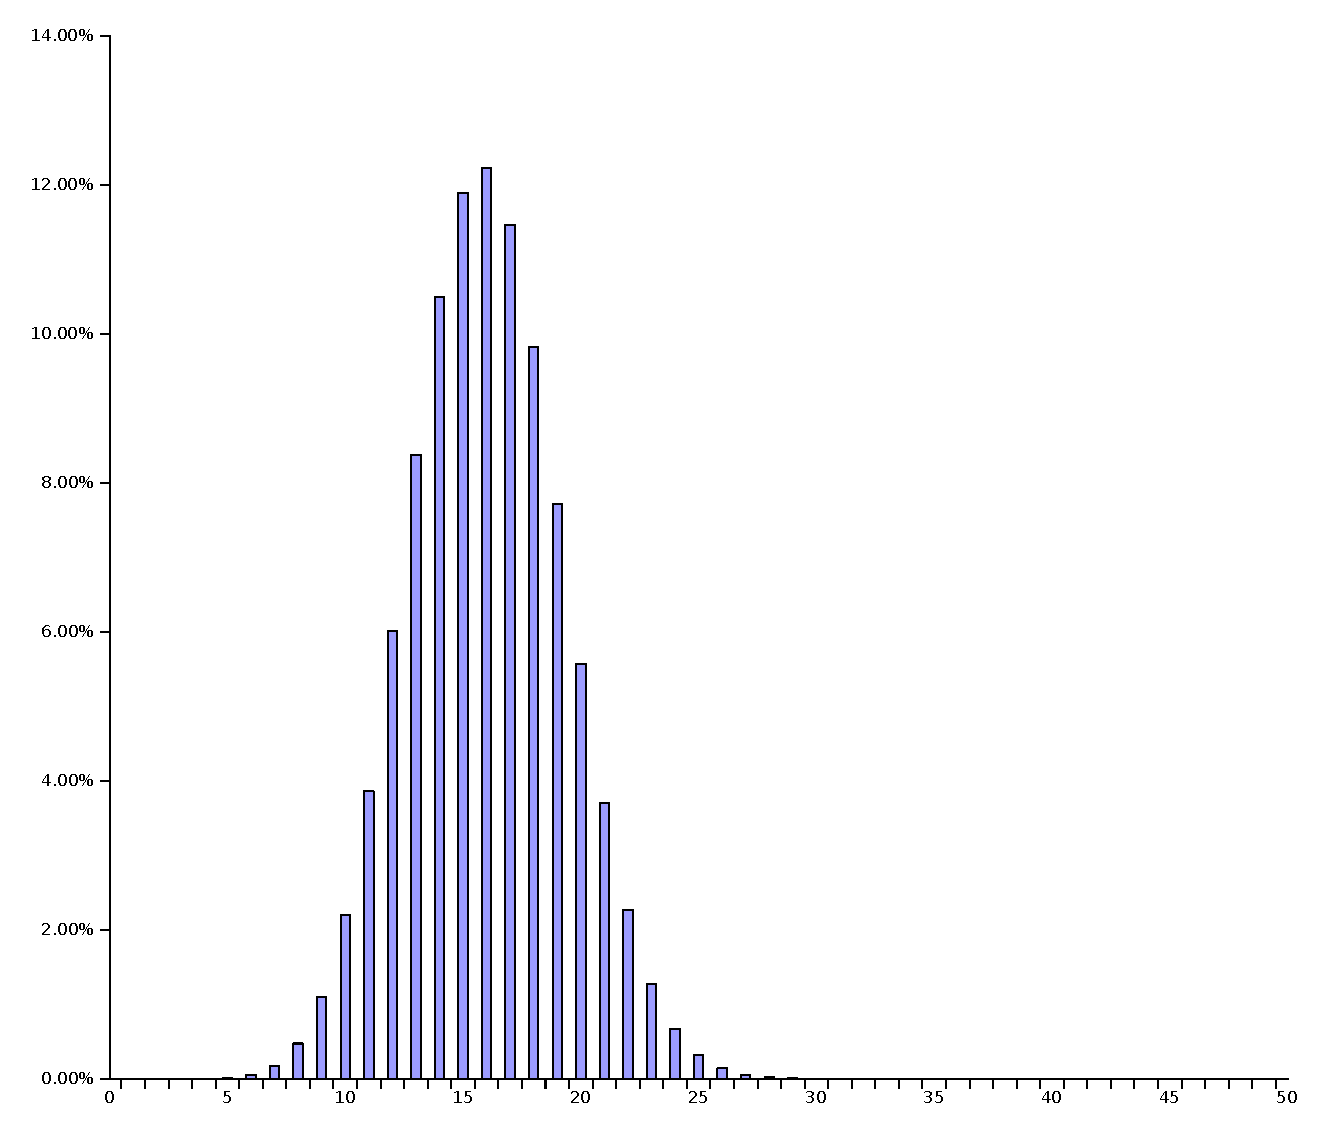
\includegraphics[scale = 0.45]{binom_dist.eps}
\caption{Binomické rozdělení - $n = 50, p = 0.30$}
\label{binom_dist}
\end{figure}
\end{center}

Člen $b(m; n, p)$ nazýváme centrálním členem. Velmi často označujeme $m$ jako nejvíce pravděpodobný počet úspěchů, nicméně je třeba mít na paměti, že pro velká $n$ jsou všechna $b(k; n, p)$ relativně malá. V navazující kapitole prokážeme, že $b(m; n, p)$ je přibližně $\frac{1}{\sqrt{2 \pi npq}}$.

Pravděpodobnost $r$ úspěchů je zpravidla méně zajímavá než pravděpodobnost nejméně $r$ úspěchů. Ta je definována jako
\begin{equation}
P[S \ge r] = \sum_{v = 0}^{\infty} b(r + v; n, p)
\end{equation}
Výše uvedená řada je nekonečná pouze zdánlivě - všechny členy pro $v > n - r$ jsou rovny nule.

Odvoďme horní limit pro (6.4). Předpokládejme, že $r > np$. Z (6.2) je zřejmé, že jednotlivé členy řady (6.4) klesají rychleji než členy geometrické posloupnosti s násobkem $1 - \frac{r - np}{rq} = \frac{p(n - r)}{rq}$. Proto platí
\begin{equation}
P[S_n \ge r] \le b(r; n, p) \frac{rq}{r - np}
\end{equation}
Protože $r > np$, existuje s ohledem na (6.3) více než $r - np$ celých čísel $k$, která splňují podmínku $m \le k \le r$. Součet odpovídajících členů binomického rozdělení je menší než jedna, přičemž žádný není menší než $b(r; n, p)$. Člen $b(r; n, p)$ je shora ohraničen $(r - np)^{-1}$, a proto
\begin{equation}
P[S_n \ge r] \le \frac{rq}{(r - np)^2}, ~~~ r > np
\end{equation}

Shodnou argumentaci je možné použít také pro situaci, kdy $r < np$. Tvrzení, že nastalo maximálně $r$ úspěchů je shodné s tvrzením, že nastalo minimálně $n - r$ neúspěchů. Vzorec (6.6) tak přejde do tvaru
\begin{equation}
P[S_n \le r] \le \frac{(n - r)p}{(np - r)^2}, ~~~ r < np
\end{equation} 

\section{Zákon velkých čísel}

Jestliže realizujeme $n$ vzájemně nezávislých a shodných pokusů, v jejichž rámci nastane $v$-krát jev $A$, intuitivně stanovíme pravděpodobnost realizace tohoto jevu na $P[A] = \frac{v}{n}$.

Analogicky označíme-li počet úspěchů v rámci $n$ Bernoulliho pokusů jako $S_n$, pak pro dostatečně velké $n$ lze očekávat, že $\frac{S_n}{n}$ se bude nacházet v blízkosti pravděpodobnosti $p$. Předpokládejme, že pravděpodobnost $\frac{S_n}{n}$ překročí $p + \epsilon$, kde $\epsilon > 0$ je libovolně malé reálné číslo. Pravděpodobnost této situace se shoduje s pravděpodobností $P[S_n > n(p + \epsilon)]$, která je dle (6.7) menší než $\frac{1}{n \epsilon^2}$. Z toho vyplývá, že s rostoucím $n$ se $P[S_n > n(p + \epsilon)]$ blíží nule. Stejně tak platí $P[S_n < n(p - \epsilon)] \rightarrow 0$, a proto
\begin{equation}
P\Bigg[ \Big| \frac{S_n}{n} - p \Big| < \epsilon \Bigg] \rightarrow 1
\end{equation}
S rostoucím $n$ se pravděpodobnost, že se průměrný počet úspěchů odlišuje od $p$ o více než stanovené $\epsilon$, blíží nule. Tato definice je jednou z forem tzv. zákona velkých čísel.

\chapter{Poissonovo rozdělení}

\section{Aproximace binomického rozdělení pomocí Poissonova rozdělení}

Řadu praktických problémů lze převést do roviny velkého počtu $n$ Bernoulliho pokusů s relativně malou pravděpodobností úspěch $p$, přičemž součin $\lambda = np$ je přiměřeného rozsahu. V těchto případech je vhodné aproximovat $b(k; n, p)$ pomocí Poissonova rozdělení. Pro $k = 0$ získáváme
\begin{equation*}
b(0; n, p) = (1 - p)^n = \Big( 1 - \frac{\lambda}{n} \Big)
\end{equation*}
Přechodem na logaritmus a s využitím Taylorova rozvoje
\begin{equation*}
\ln \frac{1}{1 - t} = t + \frac{1}{2}t^2 + \frac{1}{3}t^3 + \frac{1}{4}t^4 + ... 
\end{equation*}
získáváme
\begin{equation*}
\ln b(0; n, p) = n \ln \Big( 1 - \frac{\lambda}{n} \Big) = -\lambda - \frac{\lambda^2}{2n} - \frac{\lambda^3}{3n^2} - ...
\end{equation*}
Pro velká $n$, kdy je možné zanedbat všechny členy do řádu $n^{-1}$ včetně, tak platí $b(0; n, p) \approx e^{-\lambda}$. Z (6.2) je dále patrné, že pro libovné $k$, dostatečně velké $n$ a malou pravděpodobnost úspěchu $p$ platí
\begin{equation*}
\frac{b(k; n, p)}{b(k-1; n, p)} = \frac{\lambda - (k - 1)p}{kq} \approx \frac{\lambda}{k}
\end{equation*}
Z toho lye dovodit
\begin{equation*}
b(1; n, p) \approx \lambda b(0; n, p) \approx \lambda e^{-\lambda}
\end{equation*}
\begin{equation*}
b(2; n, p) \approx \frac{1}{2} \lambda b(0; n, p) \approx \frac{1}{2} \lambda^2 e^{-\lambda}
\end{equation*}
a obecně pomocí indukce
\begin{equation*}
b(k; n, p) \approx \frac{\lambda^k}{k!} e^{-\lambda}
\end{equation*}
Tímto jsme odvodili Poissonovu aproximaci binomického rozdělení. Pro Poissonovo rozdělení budeme používat notaci
\begin{equation*}
p(k; \lambda) = e^{-\lambda}\frac{\lambda^k}{k!}
\end{equation*}
\begin{example}
Jaká je pravděpodobnost $p_k$, že ve společnosti o 500 lidech přesně $k$ bude mít narozeniny na Nový rok? Na tento problém lze pohlížet jako na sérii 500 Bernoulliho pokusů s $p = \frac{1}{365}$. Také lze použít Poissonovu approximaci s $\lambda = \frac{500}{365} = 1.3699$.
\begin{center}
\begin{tabular}{| c | c c c c c c |}
\hline
$k$ & 0 & 1 & 2 & 3 & 4 & 5\\
\hline
Binomické rozdělení   & 0.2537 & 0.3484 & 0.2388 & 0.1089 & 0.0372 & 0.0101\\
Poissonova aproximace & 0.2541 & 0.3481 & 0.2385 & 0.1089 & 0.0373 & 0.0102\\
\hline
\end{tabular}
\end{center}
\end{example}

\begin{example}
Uvažujme výrobu šroubů, kdy každý šroub má pravděpodobnost $p = 0.015$, že bude zmetkem. Máme-li krabici obsahující 100 šroubů, pak pravděpodobnost, že neobsahuje žádný zmetek, je $(1 - 0.015)^{100} = 0.22061$. S pomocí Poissonovy aproximace získáme $e^{-1.5} = 0.22313$, což je poměrně blízké skutečné pravděpodobnosti. Položme si otázku, kolik šroubů by musela obsahovat krabice, aby pravděpodobnost výskytu alespoň 100 bezchybných šroubů byla 0.8 nebo vyšší. Je zrejmé, že krabice musí obsahovat $100 + x$ šroubů. Vzhledem k tomu, že $x$ je relativně malé, může i nadále předpokladát, že v rámci Poissonovy approximace je $\lambda = 1.5$. Hledaný počet dodatečných šroubů je pak nejmenší přirozené číslo $x$, které splňuje nerovnici
\begin{equation*}
e^{-1.5}\Big( 1 + \frac{1.5}{1} + ... + \frac{1.5^x}{x!}\Big) \ge 0.8
\end{equation*}
Tato nerovnost je splněna pro $x = 2$. Aby krabice obsahovala s pravděpodobností 80\% nejméně 100 bezchybných šroubů, musí obsahovat 102 šroubů.
\end{example}

\section{Poissonovo rozdělení}

V předchozím textu jsme dokázali, že Poissonovo rozdělení lze použít jako aproximaci pro binomické rozdělení. V kapitole (3) jsme se zabývali pravděpodobností realizace dané počtu jevů, která se opět limitně blížila Poissonově rozdělení. Poissonovo rozdělení lze tedy aplikovat při řešení široké škály problémů. Z pohledu teorie statistiky jsou vedle Poissonova rozdělení klíčové také binomické rozdělení a normální rozdělení, které si představíme v navazující kapitole.

Pravděpodobnostní rozdělení Poissonova rozdělení je
\begin{equation}
p(k; \lambda) = e^{-\lambda} \frac{\lambda^k}{k!}
\end{equation}
Součtem (7.1) přes $k = 0, 1, 2, ...$ získáme Taylorův rozvoj pro $e^{\lambda}$ vynásobený členem $e^{-\lambda}$.
\begin{equation*}
e^{\lambda} = 1 + \lambda + \frac{\lambda^2}{2!} + \frac{\lambda^3}{3!} + ...
\end{equation*}
Proto pro libovolné $\lambda$ je tento součet roven jedné.

\subsection{Distribuce v čase}

\begin{example}
Klasickým příkladem, který slouží pro ilustraci Poissonova rozdělení, je počet příchozích telefonních hovorů. Každý příchozí telefonní hovor je možné zobrazit jako bod na časové ose. Jestliže časovou osu rozdělíme na intervaly, lze počet telefonních hovorů v těchto intervalech modelovat pomocí Poissonova rozdělení.
\end{example}

Uvažujme jednotkový časový interval rozdělený na $n$ vzájemně se nepřekrývajících subintervalů délky $\frac{1}{n}$. Na množinu konečného počtu bodů, které jsou obsaženy v jednotkovém intervalu, lze pohlížet jako na výsledek náhodného procesu, který každému ze subintervalů přiřadí s pravděpodobností $p_n$ jeden nebo více těchto bodů. Každý subinterval lze tedy označit jako prázdný nebo obsazený. Za předpokladu časových subintervalů můžeme situaci modelovat pomocí Bernoulliho pokusů - pravděpodobnost obsazenosti právě $k$ subintervalů je tak rovna $b(k; n, p_n)$. Zdokonalme popisovaný diskrétní model předpokladem $n \rightarrow \infty$. Pravděpodobnost, že je celý jednotkový interval prázdný, se musí blížit limitní hodnotě. Zároveň je to také pravděpodobnost, že jsou prázdné všechny subintervaly, a proto je rovna $(1 - p_n)^n$. Tato pravděpodobnost se blíží limitní hodnotě právě tehdy a jen tehdy, jestliže se limitní hodnotě blíží také $np_n$\footnote{To lze dokázat zlogaritmováním výrazu $(1 - p_n)^n$ a následným využitím vztahu $\ln(1 + x) \approx x$.}. Možnost $n p_n \rightarrow \infty$ je vyloučena, protože by implikovala někonečně mnoho bodů v uvažované množině a to i pro sebemenší výchozí interval. Náš model vyžaduje existenci takového čísla $\lambda$, pro které platí $np_n \rightarrow \lambda$. V tomto případě lze pravděpodobnost obsazenosti právě $k$ subintervalů aproximovat pomocí $p(k; \lambda)$. Protože vzhledem k $n \rightarrow \infty$ pracujeme s jednotlivými body, odpovídá počet obsazených subintervalů počtu bodů obsažených v jednotkovém intervalu.

V praxi je častno nutné nahradit jednotkový časový interval časovým intervalem délky $t$. Tento interval opět rozdělíme na subintervaly délky $\frac{1}{n}$ a pravděpodobností obsazenosti $p_n$. Počet subintervalů je roven přirozenému číslu, které je nejbližší číslu $nt$. Přechod k limitnímu vyjádření je shodný s tím rozdílem, že $\lambda$ je nahrazeno $\lambda t$. Vzorec
\begin{equation}
p(k; \lambda t) = e^{-\lambda t} \frac{(\lambda t)^k}{k!}
\end{equation}
tak definuje pravděpodobnost nalezení $k$ bodů v intervalu délky $t$. Konkrétně pro $k = 0$ je tato pravděpodobnost rovna $e^{-\lambda t}$ a pro $k \ge 1$ je pak rovna $1 - e^{-\lambda t}$.

Na parametr $\lambda$ lze nahlížet jako na konstantu, která určuje hustotu bodů na časové ose. Čím je tento parametr vyšší, tím nižší je pravděpodobnost (7.2), že v intervalu délky $tr$ nenalezneme žádný bod. Uvažujme fyzikální experiment, ve kterém je vymezený prostor po konstantní bodu $t$ vystaven záření alfa. Přepokládejme, že je tento experiment prováděn $N$-krát a že po každém experimentu je stanoven počet alfa částic, které dosáhly vymezeného prostoru. Počet měření, ve kterých bylo napočítáno $k$ částic, označme jako $N_k$. Zcela zřejmě platí
\begin{equation*}
N_0 + N_1 + N_2 + ... = N
\end{equation*}
Celkový počet částic pozorovaných během všech experimentů je roven
\begin{equation}
N_1 + 2N_2 + 3N_3 + ... = T
\end{equation}
Průměrný počet částic na pozorování je tedy roven $\frac{T}{N}$. Jestliže je $N$ dostatečně veliké, lze očekávat
\begin{equation}
N_k \approx Np(k; \lambda t)
\end{equation}
Dosazením (7.4) do (7.3) získáme
\begin{equation}
T \approx N(p(1; \lambda t) + 2p(2; \lambda t) + 3p(3; \lambda t) + ...) = Ne^{-\lambda t} \lambda t \Big(1 + \frac{\lambda t}{1} + \frac{(\lambda t)^2}{2!} + ... \Big) = N \lambda t
\end{equation}
a proto
\begin{equation}
\lambda t \approx \frac{T}{N}
\end{equation}
Tento vztah nám umožňuje odhad $\lambda$ na základě pozorování.

\subsection{Distribuce v rovině popř. prostoru}

Ve výše uvedeném textu jsme uvažovali distribuci bodů podél časové osy. Stejnou logiku však lze aplikovat také na distribuci bodů v rovině popř. prostoru. Namísto časového intervalu délky $t$, budeme uvažovat výseky z roviny popř. prostoru o ploše popř. objemu $t$. Základním předpokladem pak bude, že pravděpodobnost nalezení $k$ bod; v daném výseku se odvíjí pouze od jeho plochy popř. objemu. Ostatní předpoklady zůstávají - (a) jestliže je $t$ dostatečně malé, je pravděpodobnost nalezení více než jednoho bodu ve výseku zanedbatelná a (b) jednotlivé výseky se nepřekrývají a lze je považovat za vzájemně nezávislé.

\begin{example}
Klasickým příkladem aplikace Poissonova rozdělení na rovinný útvar je počet bakterií v Petriho misce, kdy je miska rozdělena na řadu malých čtverců, ve kterých je následně stanovován počet bakterií.
\end{example}

\section{Negativní binomické rozdělení}

Uvažujme posloupnost Bernoulliho pokusů. Kolik pokusů je třeba realizovat, než se dostaví $r$-tý úspěch? Protože platí $v \ge r$, používá se vztah $v = k + r$. Pravděpodobnost, že $r$-tý úspěch nastane během pokusu $r + k$, označme jako $f(k; r, p)$. Tato pravděpodobnost je rovna pravděpodobnosti, že přesně $k$ neúspěchů předchází $r$-tému úspěchu. K této situaci dojde tehdy a jen tehdy, když mezi prvními $r + k - 1$ pokusy nastane přesně $k$ neúspěchů a poslední $r+k$-tý pokus je úspěch. Odpovídající pravděpodobnost je rovna
\begin{equation}
f(k; r, p) = \binom{r + k - 1}{k}p^rq^k
\end{equation}
popř. ji lze s využitím vztahu
\begin{equation*}
\binom{-a}{k} = (-1)^k \binom{a + k - 1}{k}, ~~~ a > 0
\end{equation*}
upravit do podoby
\begin{equation}
f(k; r, p) = \binom{-r}{k} p^r (-q)^k
\end{equation}
Předpokládejme, že Bernoulliho pokusy jsou prováděny tak dlouho, pokud nenastane $r$-tý úspěch. Položme si otázku, zda může nastat situace, kdy Bernoulliho pokusy budou prováděny nekonečně dlouho, aniž by nastal $r$-tý úspěch. Pravděpodobnost $\sum_{k = 0}^{\infty} f(k; r, p)$ vyjadřuje situaci, kdy $r$-tý úspěch nastane po konečném počtu Bernoulliho pokusů. Možnost nekonečné posloupnosti Bernoulliho pokusů můžeme zavrhnout za předpokladu, že platí
\begin{equation}
\sum_{k = 0}^{\infty} f(k; r, p) = 1
\end{equation}
To platí, protože vzhledem k (7.8) lze (7.9) vyjádřit jako
\begin{equation*}
\sum_{k = 0}^{\infty} \binom{-r}{k}p^r(-q)^k = p^r(1 - q)^{-r} = p^r p^{-r} = 1 
\end{equation*}
\begin{theorem}
Pro libovolné reálné $r > 0$ a pravděpodobnost úspěchu $0 < p < 1$ nazýváme $f(k; r, p)$, které je definovano dle (7.7) resp. (7.8), pravděpodobnostním rozdělením negativního binomického rozdělení\footnote{V některých publikacích se můžeme setkat s označením Pascalovo rozdělení.}. Pravděpodobnost $f(k; r, p)$ lze interpretovat jako počet pokusů potřebných k dosažení $r$-tého úspěchu.
\end{theorem}
\begin{example}
Byl jednou jeden matematik, který nosil jednu krabičku zápalek v právé a jednu krabičku zápalek v levé kapse kalhot. Vždy když si chtěl zapálit, náhodně sáhl do jedné z krabiček a vytáhl z ní zápalku. Přepokládejme, že na začátku obsahovala každá krabička $N$ zápalek. Uvažujme situaci, kdy matematik šáhne do krabičky v levé kapse a zjistí, že je prázdná. Druhá z krabiček v ten okamžik obsahuje obsahuje $0 < r \le N$u zápalek. Aby tato situace nastala, musel matematik sáhnout $(N + 1)$-krát do levé kapsy a $(N - r)$-krát do pravé kapsy. Pravděpodobnost, že tato situace nastane, je rovna $f(N - r; N + 1, \frac{1}{2})$. A protože měl dvě kapsy, pak pravděpodobnost, že šáhl do prázdné krabičky, přičemž druhá krabička obsahovat $r$ zápalek, je rovna $2f(N - r; N + 1; \frac{1}{2}) = \binom{2N - r}{N}2^{-2N + r}$.
\end{example}

\section{Multinomické rozdělení}

Binomické rozdělení může být snadno zobecněno pro $n$ nezávislých pokusů z nichž každý může mít více než dva výstupy. Označme jednotlivé možné výstupu každého z pokusů jako $E_1$, $E_2$, ..., $E_r$ a předpokládejme, že pravděpodobnost realizace $E_i$ je $p_i$. Je zřejmé, že musí platit $p_1 + ... + p_r = 1$. Výstup $n$ pokusů pak má podobu $E_3E_1E_2 \dotsm$. Pravděpodobnost, že rámci $n$ pokusů nastane $E_1$ právě $k_1$-krát, $E_2$ právě $k_2$-krát, $E_3$ právě $k_3$-krát atd., je rovna
\begin{equation}
\frac{n!}{k_1! k_2! \dotsm k_r!} p_1^{k_1} p_2^{k_2} p_3^{k_3} \dotsm p_r^{k_r}
\end{equation}
kde $k_1 + k_2 + ... + k_r = n$.

Rovnici (7.10) nazýváme multinomickým rozdělením, protože její pravá strana je obecným členem multinomického rozvoje výrazu $(p_1 + ... + p_r)^n$. Hlavní oblast použití multinomického rozdělení zahrnuje výběry s vracením, kdy jsou jednotlivé prvky výběru rozděleny do vícero skupin.

\begin{example}
Uvažujme hod dvanácti hracími kostkami. Jaká je pravděpodobnost, že každé číslo padne právě dvakrát? V tomto případě představují $E_1$, ..., $E_6$ strany hrací kostky a všechna $k_i$ jsou rovna dvěma a všechna $p_i$ rovna $\frac{1}{6}$. Námi hledaná pravděpodobnost je tedy rovna $\frac{12!}{(2!)^6}\frac{1}{6^{12}} = 0.0034$.
\end{example}

\chapter{Normální rozdělení jako aproximace binomického rozdělení}

\section{Normální rozdělení}

\begin{definition}
Funkci
\begin{equation}
\mathfrak{n}(x) = \frac{1}{\sqrt{2 \pi}} e^{-\frac{1}{2}x^2}
\end{equation}
nazýváme funkcí hustoty normálního rozdělení. Integrál této funkce
\begin{equation}
\mathfrak{N}(x) = \frac{1}{\sqrt{2 \pi}} \int_{-\infty}^x e^{-\frac{1}{2}y^2}dy
\end{equation}
pak nazýváme distribuční funkcí normálního rozdělení.
\end{definition}
\begin{center}
\begin{figure}
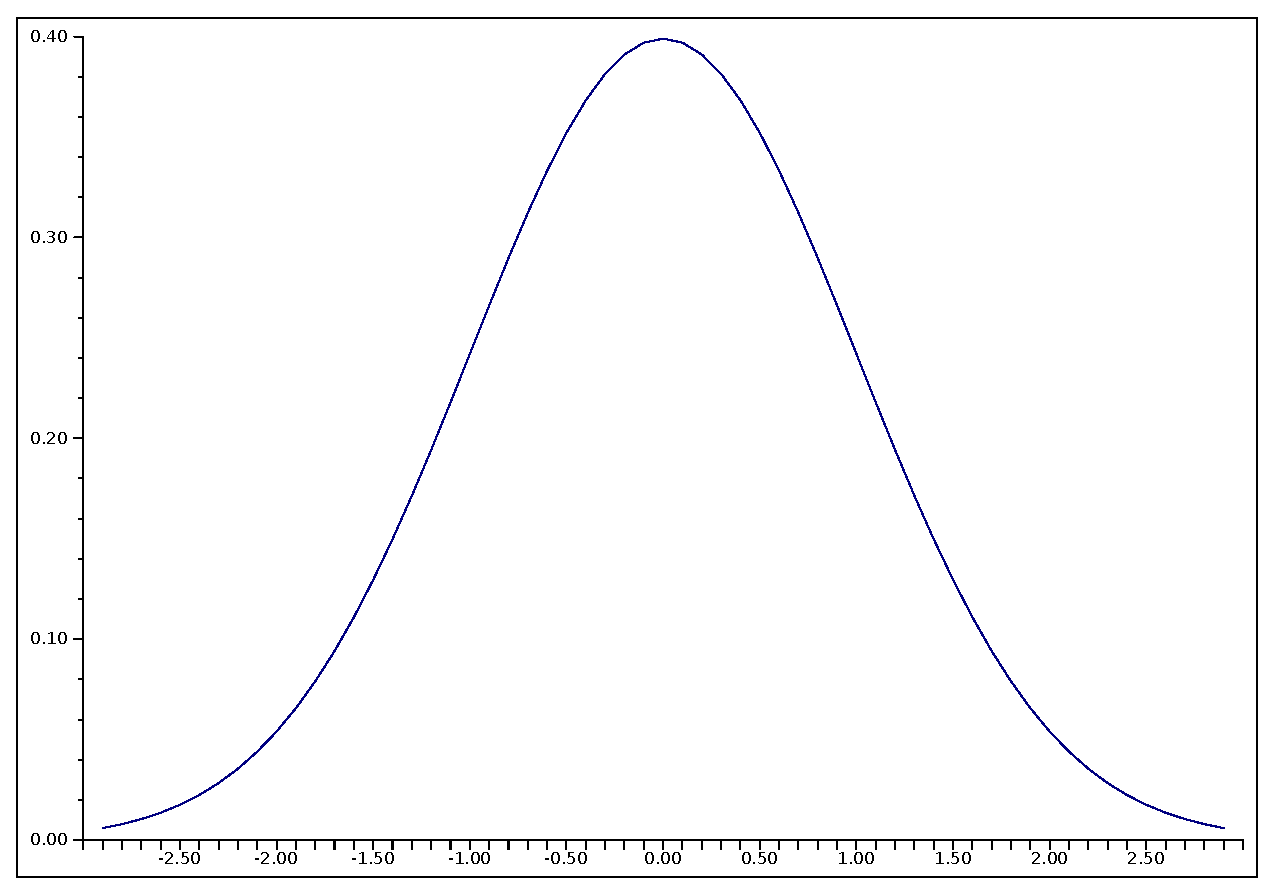
\includegraphics[scale = 0.45]{norm_dens_fce.eps}
\caption{Funkce hustoty $\mathfrak{n}(x)$ normálního rozdělení}
\label{norm_dens_fce}
\end{figure}
\end{center}
\begin{center}
\begin{figure}
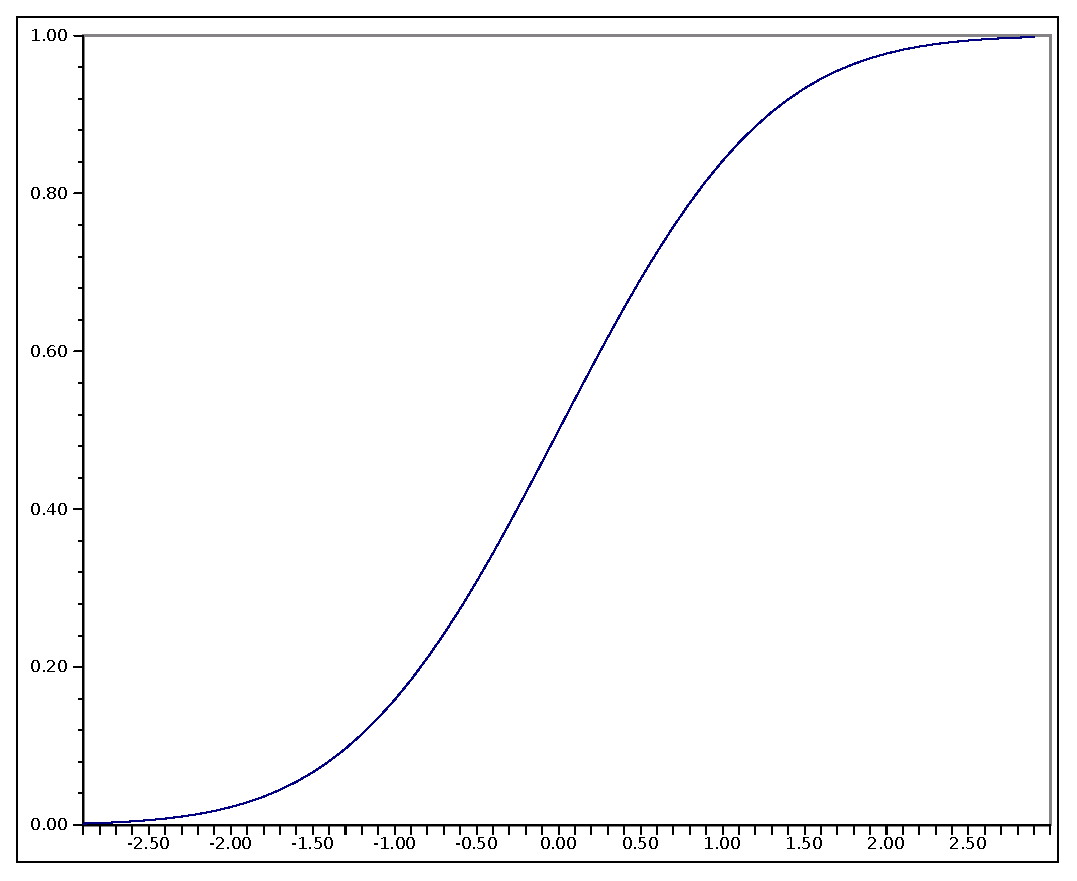
\includegraphics[scale = 0.45]{norm_dist_fce.eps}
\caption{Distribuční funkce $\mathfrak{N}(x)$ normálního rozdělení}
\label{norm_dist_fce}
\end{figure}
\end{center}
Graf funkce $\mathfrak{n}(x)$ má zvonu, který je symetrický kolem bodu nula, kde dosahuje maxima $\frac{1}{\sqrt{2 \pi}} = 0.399$.
\begin{lemma}
Plocha vymezená osou $x$ a křivkou $\mathfrak{x}(x)$ je rovna jedné.
\end{lemma}
\begin{proof}
Platí
\begin{equation*}
\Big( \int_{-\infty}^{\infty} \mathfrak{n}(x) \Big)^2 = \int_{-\infty}^{\infty} \int_{-\infty}^{\infty} \mathfrak{n}(x)\mathfrak{n}(y)dx dy = \frac{1}{2 \pi} \int_{-\infty}^{\infty} \int_{-\infty}^{\infty} e^{-\frac{1}{2}(x^2 + y^2)}dx dy
\end{equation*}
Takto odvozený dvojitý integrál lze vyjádřit pomocí polárních souřadnic.
\begin{equation*}
\frac{1}{2 \pi} \int_0^{2 \pi} \int_0^{\infty} r e^{-\frac{1}{2}r^2} dr d \theta = 1
\end{equation*}
Tímto jsme dokázali výše uvedenou lemu.
\end{proof}
Z definice (8.1.1) a z lemy (8.1.1) vyplývá, že funkce $\mathfrak{N}(x)$ rostoucí funkce, která postupně nabývá hodnot od nuly do jedné. Pro tuto funkci platí
\begin{equation}
\mathfrak{N}(-x) = 1 - \mathfrak{N}(x)
\end{equation}

V řadě případů je vhodné mít odhad konce pravděpodobnostního rozdělení $1 - \mathfrak{N}(x)$ pro velká $x$.
\begin{lemma}
Pro $x \rightarrow \infty$ platí
\begin{equation*}
1 - \mathfrak{N}(x) \sim x^{-1} \mathfrak{n}(x)
\end{equation*}
Přesněji, dvojitá nerovnost
\begin{equation}
(x^{-1} - x^{-3})\mathfrak{n}(x) < 1 - \mathfrak{N}(x) < x^{-1}\mathfrak{n}(x)
\end{equation}
platí pro všechna $x > 0$.
\end{lemma}
\begin{proof}
Je zřejmé, že platí
\begin{equation*}
(1 - 3x^{-4}) \mathfrak{n}(x) < \mathfrak{n}(x) < (1 + x^{-2}) \mathfrak{n}(x)
\end{equation*}
Jednotliví členové této nerovnosti jsou záporné derivace členů v rovnici (8.4).
\end{proof}

\section{Orientace - symetrické distribuce}

V této kapitole si vysvětlíme použití normálního rozdělení jako aproximace pro binomické rozdělení s $p = \frac{1}{2}$. Existují dva důvody, proč si vybrat $p = \frac{1}{2}$. Prvním z jich je ten, že navazující výpočty jsou jednodušší a tím pádem vhodnější pro pochopení problematiky. Druhým důvodem je, že $p = \frac{1}{2}$ definuje tzv. náhodnou procházku, která je klíčová pro oblast financí.

Uvažujme sudý počet pokusů $n = 2v$ a definujme
\begin{equation*}
a_k = b(v + k; 2v, \frac{1}{2})
\end{equation*}
kde $a_k$ představuje člen ve zdálenosti $k$ od centrálního členu $a_0$ symetrického binomického rozdělení. Parametr $k$ tak nabývá hodnot od $-v$ do $v$. Protože $a_{-k} = a_{k}$, budeme se zabývat pouze členy $k \ge 0$.
\end{document}


